\documentclass[a4paper]{scrartcl}

\usepackage[
fancytheorems, 
fancyproofs, 
noindent, 
%  spacingfix,  
]{adam}

\usepackage{tikz}
\usepackage{cancel}
\usepackage{bm}

% code for adding arrows to plots
\usetikzlibrary{decorations.markings,arrows}

\title{Variational Principles}
\author{Adam Kelly (\texttt{ak2316@cam.ac.uk})}
\date{\today}


\allowdisplaybreaks

\begin{document}

\maketitle

From finding geodesics to expressing the fundamental laws of nature, variational principles and the calculus of variations arise naturally in pure \& applied mathematics, and theoretical physics.
Here, we will study such ideas, with the underlying goal of considering problems involving minimizing (or maximizing) quantities that depend on an entire function. 

This article constitutes my notes for the `Variational Principles' course, held in Easter 2021 at Cambridge. These notes are \emph{not a transcription of the lectures}, and differ significantly in quite a few areas. Still, all lectured material should be covered.

% {\color{purple}Currently up to lecture 1.}

\tableofcontents

\section{Introduction}


% Lecture 1

We will begin our study of variational principles by getting a feel for the type of problems that we care about. 
As a field, the study of variational principles can be traced back to a single problem, posed by Johann Bernoulli in 1696. It is there that we will begin.

\subsection{A Motivating Problem -- The Brachistochrone}

One of the earliest problems in the calculus of variations is the \vocab{Brachistochrone} problem.

\begin{example}[Brachistochrone]
	Consider a particle sliding on a wire between two fixed points $A$ and $B$, under the influence of gravity. Which shape of the wire will give the shortest travel time, when the particle starts from rest?
\end{example}

It is not immediately obvious what the answer to this problem is. We won't solve it right now, but we can still can take some steps in the right direction. We first setup a coordinate system, setting $A$ to be the origin, and $B$ to be some point $(x_2, y_2)$.

\begin{center}
	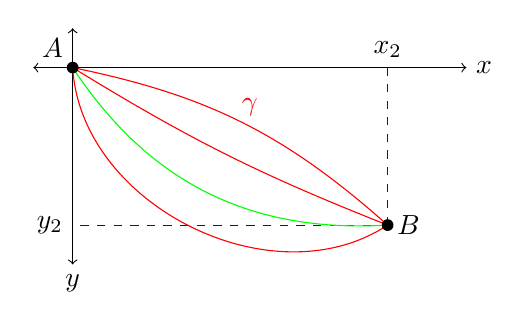
\begin{tikzpicture}
		\coordinate (origin) at (0,0);
		\coordinate (b) at (4.0, -2.0);
		
		% \filldraw[color=blue!80, fill=blue!2] (z1) circle (0.7);

		% draw axes
		\draw [<->] (-0.5, 0) -- (5.0, 0) node [right] {$x$};
		\draw [<->] (0, 0.5) -- (0, -2.5) node [below] {$y$};
	
		\draw [dashed, blue] (b) -- (4.0, 0) node [black, above] {$x_2$};
		\draw [dashed, blue] (b) -- (0, -2.0) node [black, left] {$y_2$};

		% draw some paths between A and B
		\draw [green] (origin) to [bend right=30] (b);
		\draw [red] (origin) to [bend right=60] (b);
		\draw [red] (origin) to [bend right=5] (b);
		\draw [red] (origin) to [bend left=15] (b);

		\draw (2.25, -0.5) node [red] {$\gamma$};
		% \draw plot [smooth, red] coordinates {(0,0) (2.0, -1.2) (4.0, -2.0))};

		% draw the points A and B
		\node at (b)[circle,fill,inner sep=1.5pt]{};
		\draw (b) node [right] {$B$};

		\node at (origin)[circle,fill,inner sep=1.5pt]{};
		\draw (origin) node [above left] {$A$};

		% draw vectors
		% \draw [->] (origin) -- (z1) node [anchor=south west] {$c$};
		% \draw [dashed] (1, 1.25) -- (0.3, 1.25) node [pos=0.5, anchor=south] {$\rho$};
		\end{tikzpicture}
\end{center}

In this coordinate system, for a given curve $\gamma$, we can write down the travel time 
$$
T = \int_\gamma \dd t = \int_\gamma \frac{1}{v} \dd s,
$$
where $v$ is the velocity of the particle. Since the particle starts at $y = 0$, conservation of energy implies that 
\begin{align*}
	\frac{1}{2}m v^2 + mg y &= 0 \\
	\implies v &= \sqrt{-2gy}.
\end{align*}
Thus to solve our problem, we really want to minimize
$$
T[y] = \frac{1}{\sqrt{2g}} \int_0^{x_2} \frac{\sqrt{1 + (y')^2}}{\sqrt{-y}} \dd x,
$$
subject to $y$ being a smooth function with $y(0) = 0$, and $y(x_2) = y_2$.

\subsection{Problems of Interest}

Let's jump to another problem from pure mathematics, finding geodesics.

\begin{example}[Geodesic Problem]
	Find the shortest path $\gamma$ between two points on a surface $\Sigma$ (if one exists).
\end{example}


If $\Sigma$ is $\R^2$, we can again adopt a coordinate system, and try to find the shortest curve $\gamma$ between the two points $A = (x_1, y_1)$ and $B=(x_2, y_2)$.
To solve this problem, we really want to minimize
$$
D[y] = \int_{x_1}^{x_2} \sqrt{1 + (y')^2} \dd{x},
$$
subject to $y$ being a smooth function with $y(x_1) = y_1$ and $y(x_2) = y_2$.

Both of these problems have a similar flavour: we are trying the minimize or maximize something like
\begin{equation}\label{eq:functional}
	F[y] = \int_{x_1}^{x_2} f(x, y(x), y'(x)) \dd x, \tag{$*$}
\end{equation}
among all functions such that $y(x_1) = y_1$ and $y(x_2) = y_2$.
This quantity \eqref{eq:functional} is called a \vocab{functional}, that is, a function on the space of functions\footnote{In standard calculus, we usually consider functions which map numbers $\rightarrow$ numbers. In the calculus of variations, we consider \emph{functional} which map functions $\rightarrow$ numbers. An intuitive example is that of arc-length, which takes some curve and gives back a number corresponding to its length.}.

In this article, we are going to study the \emph{calculus of variations}, in which we will be finding extrema (minima, maxima, and saddle points) of functionals. 
We will start by looking back at and extending our knowledge of extrema in finite dimensions, before using this knowledge to approach problems involving functionals.

\begin{notation}
	Throughout this article, we will frequently refer to different spaces of functions. We will let $C(\R)$ be the space of continuous functions on $\R$, and $C^k(\R)$ be the space of functions with continuous $k$th derivative. We will also write $C_{(\alpha, \beta)}^k(\R)$ for the subset of functions $f$ with $f(\alpha) = f(\beta)$.
\end{notation}

Being careful about the space of functions we work in matters more than it might first appear. Just as in real analysis, where the domain of a function has to be specified before we can sensibly ask whether it attains a maximum, here we have to say which functions are `admissible' before asking for the best one. Most of the time this will be some class of smooth functions with prescribed values at the endpoints, and we will not belabour the point -- but the reader should be aware that some of the more delicate questions in this subject (does a minimiser exist at all?) are questions about the choice of function space, and are well beyond the scope of this article.

\subsection{Variational Principles in Nature}

The phrase `variational principle' refers to something slightly more specific than the calculus of variations: it is the assertion that some \emph{law of nature} can be recast as the statement that a certain functional is stationary. This is a remarkable state of affairs, and it will be a recurring theme in what follows.

The oldest example is Fermat's principle, which we will meet properly in \autoref{sec:fermat}.

\begin{law}[Fermat's Principle]
	Light travelling between two points takes the path which requires the least time.
\end{law}

From this single sentence one can derive the law of reflection and Snell's law of refraction, both of which were discovered empirically long before. Far more striking is that \emph{all} of classical mechanics can be phrased this way.

\begin{law}[Principle of Least Action]
	A particle moving in a potential $V$ with kinetic energy $T$ travels between two fixed points in such a way that the \vocab{action}
	$$
	S[\vv{x}] = \int_{t_1}^{t_2} (T - V) \dd t
	$$
	is stationary.
\end{law}

We will see in \autoref{sec:hamilton} that this is exactly equivalent to Newton's second law. It is worth pausing on how strange this is. Newton's law is `local' in time: it tells the particle how to accelerate right now, given the force right now. The principle of least action is `global': it compares entire histories of the particle, from $t_1$ to $t_2$, and picks out the one which is stationary. That these two descriptions agree is not obvious, and the machinery we are about to develop is precisely what makes the equivalence work.

There is a further payoff. Once a physical law is written as a variational principle, the \emph{symmetries} of the functional turn directly into conserved quantities -- this is Noether's theorem, which we will prove in \autoref{sec:noether}. Conservation of momentum, angular momentum and energy all fall out of the invariance of the action under translations, rotations, and time-shifts respectively. This is by some distance the most efficient route to the conservation laws.

% Lecture 2

\section{Calculus for Functions on \texorpdfstring{$\R^n$}{R-n}}

For this section, we are going to consider a function $f \in C^2(\R^n)$, that is, $f: \R^n \rightarrow \R$, with continuous second derivative.

\subsection{Stationary Points}

Recall the definition of a stationary point for a function $f \in C^2(\R^n)$.

\begin{definition}[Stationary Point]
	We say that $a \in \R^n$ is a \vocab{stationary point} of $f$ if
	$\nabla f(a)= 0$.
\end{definition}

If $a$ is a stationary point of $f$, then we can look at the Taylor expansion of $f$ around $a$ to determine the nature of the stationary point. For $x$ near $a$, using the summation convention we have
$$
f(x) = f(a) + \cancel{(x - a) \cdot \nabla f(a)} + \frac{1}{2}(x_i - a_i)(x_j - a_j) \left.\partial^2_{ij} f \right|_a + O(|x - a|^3),
$$
where $\partial_i f = \partial f/\partial x_i$, and the linear term dies precisely because $a$ is stationary. So near a stationary point, the entire behaviour of $f$ is controlled by a quadratic form.

Now let $H_{ij} = \partial^2_{ij} f$ be the \vocab{Hessian} matrix, which we note is symmetric since $f \in C^2$. If we shift the origin such that $a = 0$ and write $H = H(0)$, then being real symmetric it can be diagonalized by an orthogonal matrix $R$, giving
$$
H' = R^T H(0) R = \begin{pmatrix}
	\lambda_1 & \cdots & 0 \\
	\vdots& \ddots &\vdots \\
	0 &\cdots & \lambda_n
\end{pmatrix}.
$$
Writing $x' = R^T x$ for the coordinates in this new (rotated) frame, we have
$$
	f(x') - f(0) = \frac{1}{2}\sum_{i = 1}^n \lambda_i (x_i')^2 + O(|x'|^3).
$$

The behaviour then depends on whether the eigenvalues of $H(0)$ are positive or negative:

\begin{enumerate}[label=(\roman*)]
	\item If all $\lambda_i > 0$, then $f(x') > f(0)$ in all directions, and we have a local minimum.
	\item If all $\lambda_i < 0$, then $f(x') < f(0)$ in all directions, and we have a local maximum.
	\item If some of the eigenvalues are positive and some are negative, then $f(x')$ is increasing in some directions and is decreasing in others, and we have a saddle point.
	\item If some (or all) of the eigenvalues are $0$, then we need to consider higher order derivatives in the Taylor expansion.
\end{enumerate}

In the special case where $n = 2$, then $\det H = \lambda_1 \lambda_2$ and $\tr H = \lambda_1 + \lambda_2$. From this we obtain the conditions:


\begin{itemize}
	\item If $\det > 0, \tr > 0$ we have a local minimum.
	\item If $\det > 0, \tr < 0$ we have a local maximum.
	\item If $\det < 0$ we have a saddle point.
	\item If $\det = 0$, then we need to look at higher derivatives.
\end{itemize}

\begin{remark}
	If a function $f: D \rightarrow \R$ is defined on some domain $D$, then the minimum or maximum could be obtained on the boundary of $D$, where we may not have $\nabla f = 0$.
	This is an easy thing to forget, and it will come back in a rather more dramatic form later on when we look at soap films.
\end{remark}

Here is a pretty application of the $n = 2$ criteria. Suppose $f: D \to \R$ is \vocab{harmonic} on $D \subseteq \R^2$, meaning $\nabla^2 f = f_{xx} + f_{yy} = 0$. Then $\tr H = 0$ everywhere, so at any stationary point either both eigenvalues vanish or they have opposite signs. Hence a non-constant harmonic function has no interior maxima or minima at all: its extreme values are attained on $\partial D$. This is the \emph{maximum principle}, which the reader may have seen in complex analysis.

\begin{example}[Finding and Classifying Stationary Points]
	Consider the function $f(x, y) = x^3 + y^3 - 3xy$. Then at a stationary point we have
	$$
\nabla f = \begin{pmatrix}
	3x^2 - 3y \\
	3y^2 - 3x
\end{pmatrix} = \begin{pmatrix}
	0 \\ 0
\end{pmatrix}.
	$$
	These imply that at a stationary point, $y^4 = y$. Thus we have the points $(0, 0)$ and $(1, 1)$. We can write down the Hessian as
	$$
	H = \begin{pmatrix}
		6x & -3 \\ -3 & 6y
	\end{pmatrix}.
	$$
	At $(0, 0)$, we have $\det H = -9 < 0$, so $f$ has a saddle point there. At $(1, 1)$, we have $\det H = 27 > 0$, and $\tr H = 12 > 0$, so $f$ has a local minimum there.
\end{example}

The degenerate case really does need care, as the following pair shows.

\begin{example}[Degenerate Hessians]
	Consider $f(x, y) = x^4 + y^4$ and $g(x, y) = x^4 - y^4$. Both have their only stationary point at the origin, and for both the Hessian there is the zero matrix, so $\det H = \tr H = 0$ and our criteria say nothing at all. But $f$ clearly has a global minimum at the origin, while $g$ has a saddle: it increases along the $x$-axis and decreases along the $y$-axis. There is no way to tell these apart without looking at the fourth-order terms.

	This is exactly analogous to the one-dimensional situation, where $f''(0) = 0$ leaves us unable to distinguish $x^4$ from $x^3$ from $-x^4$.
\end{example}

\subsection{Constraints and Lagrange Multipliers}\label{sec:lm}

Consider the following problem, and two natural ways to solve it.

\begin{example}
	Find the circle centered at $(0, 0)$ with smallest radius such that the circle intersects the parabola $y = x^2 - 1$.
\end{example}

\emph{Direct Solution.} One way to solve this problem is to substitute the constraint $y = x^2 - 1$ into the expression we are trying to minimize.
$$
r^2 = x^2 + y^2 = x^2 + (x^2 - 1)^2 = x^4 - x^2 + 1.
$$
To have a stationary point, the derivative of the RHS must be zero, so $4x^3 - 2x = 0$. This gives us two solutions: $x = \pm 1/\sqrt{2}, y = - 1/2$ and $x = 0, y = -1$. These give the two possible radii of $\sqrt{3}/2$ and $1$, of which the first is the smallest.

While this solution works, it's not hard to imagine that we may not be able to solve the constraint for $y$ -- and even when we can, doing so may destroy a symmetry of the problem which we would rather keep. An alternate solution is given below.

\emph{Lagrange Multipliers Solution.} Define the function $h(x, y, \lambda) = f(x, y) - \lambda g(x, y)$, where $f(x, y) = x^2 + y^2 = r^2$, $g(x, y) = 0$ is the constraint, and $\lambda$ is the Lagrange multiplier. So $h = x^2 + y^2 - \lambda (y - x^2 + 1)$. We are going to extremize this over $3$ variables with no constraints.
\begin{align*}
	\frac{\partial h}{\partial x} &= 2x + 2 \lambda x = 0, \\
	\frac{\partial h}{\partial y} &= 2y - \lambda  = 0, \\
	\frac{\partial h}{\partial \lambda} &= -(y - x^2 + 1) = 0,
\end{align*}
where the third condition is exactly our constraint -- this is the small miracle that makes the method work. From the first equation, either $x = 0$ or $\lambda = -1$. From these we get either $x = 0, y = -1$ with $f = 1, \lambda = -2$, or $y = -1/2, x = \pm 1/\sqrt{2}$ with $f = 3/4, \lambda = -1$, giving the radius $\sqrt{3}/2$ as before.

So why does the second solution work? Well suppose that we wanted to minimize a function $f$ subject to $g = 0$. Then $\nabla g$ is perpendicular to the level set $g = 0$. Also, $\nabla f$ is perpendicular to the level set $f(x) = c$, for any constant $c$. Now imagine walking along the constraint curve. As long as $\nabla f$ has a nonzero component \emph{along} the curve, we can decrease $f$ by taking a step in the appropriate direction, and so we are not at an extremum. So at the extremum $\nabla f$ must be entirely perpendicular to the constraint curve; that is, parallel to $\nabla g$, so
$$
\nabla f - \lambda \nabla g = 0,
$$
for some $\lambda$. Equivalently, the level curve of $f$ through the extremum is \emph{tangent} to the constraint curve. Thus it suffices to consider the extrema of $h = f - \lambda g$.

\begin{center}
	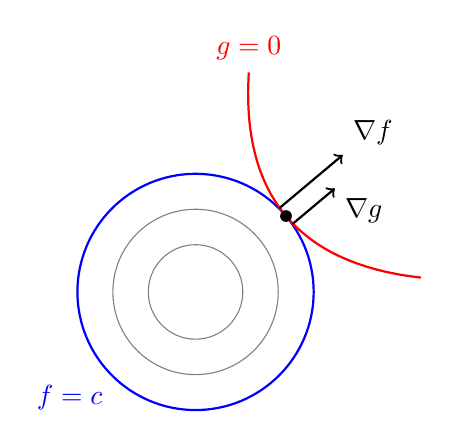
\begin{tikzpicture}[scale=1.0]
		% level curves of f (circles centred at origin)
		\draw [thin, gray] (0,0) circle (0.6);
		\draw [thin, gray] (0,0) circle (1.05);
		\draw [thick, blue] (0,0) circle (1.5);

		% constraint curve g = 0, tangent to the circle of radius 1.5 at 40 degrees
		\draw [thick, red] plot [smooth] coordinates {(2.862,0.182) (2.635,0.213) (2.420,0.255) (2.218,0.307) (2.028,0.370) (1.850,0.443) (1.685,0.526) (1.533,0.620) (1.392,0.725) (1.265,0.839) (1.149,0.964) (1.046,1.100) (0.955,1.245) (0.877,1.402) (0.811,1.568) (0.758,1.745) (0.717,1.933) (0.688,2.131) (0.672,2.339) (0.668,2.558) (0.676,2.787)};
		\node [red, above] at (0.676, 2.82) {$g = 0$};

		% tangency point
		\node at (1.149, 0.964) [circle, fill, inner sep=1.5pt] {};

		% gradients at the tangency point (both along the common normal)
		\draw [->, thick] (1.065, 1.064) -- (1.869, 1.739) node [above right] {$\nabla f$};
		\draw [->, thick] (1.233, 0.864) -- (1.769, 1.314) node [below right] {$\nabla g$};

		\node [blue, below left] at (-1.06, -1.06) {$f = c$};
	\end{tikzpicture}
\end{center}

This picture also tells us when the method can fail: if $\nabla g = 0$ at the extremum, then $\nabla f = \lambda \nabla g$ carries no information. Such points are called \emph{singular} and have to be checked separately.

This method generalizes to multiple variables and multiple constraints. For example, if we wanted to extremize $f: \R^n \rightarrow \R$, subject to $g_{\alpha}(x) = 0$, where $g_{\alpha}: \R^n \rightarrow \R$ and $\alpha = 1, \dots, k$, we would define
$$
h(x_1, \dots, x_n, \lambda_1, \dots, \lambda_k) = f - \sum_{\alpha=1}^k \lambda_{\alpha} g_{\alpha},
$$
and would extremize this function with respect to the $n + k$ variables. Geometrically, the constraints $g_\alpha = 0$ cut out an $(n-k)$-dimensional surface, and the condition is that $\nabla f$ lies in the span of the normals $\nabla g_1, \dots, \nabla g_k$, that is, $\nabla f$ has no component tangent to the surface.

\begin{example}[Two Constraints]
	Let us maximize $f(x, y, z) = x + y + z$ on the circle cut out of the unit sphere by the plane $z = \frac{1}{2}$. So we take
	$$
	g_1 = x^2 + y^2 + z^2 - 1, \qquad g_2 = z - \tfrac{1}{2},
	$$
	and set $h = f - \lambda g_1 - \mu g_2$. Then
	$$
	\frac{\partial h}{\partial x} = 1 - 2\lambda x = 0, \quad \frac{\partial h}{\partial y} = 1 - 2 \lambda y = 0, \quad \frac{\partial h}{\partial z} = 1 - 2 \lambda z - \mu = 0,
	$$
	together with the two constraints. The first two give $x = y = 1/(2\lambda)$, and the constraints then give $2x^2 = 1 - z^2 = 3/4$, so $x = y = \pm\sqrt{3}/(2\sqrt{2})$. The maximum is at the positive root, where
	$$
	f = \frac{\sqrt{3}}{\sqrt{2}} + \frac{1}{2} = \sqrt{\tfrac{3}{2}} + \tfrac{1}{2}.
	$$
	Note that $\mu$ was never needed: it only served to absorb the fact that the $z$-equation is not required to balance. This is typical -- the multipliers are auxiliary unknowns which we are free to discard once they have done their job.
\end{example}

Although we have been treating $\lambda$ as a bookkeeping device, it does have a meaning, and a rather useful one.

\begin{proposition}[The Meaning of the Multiplier]
	Suppose we extremize $f$ subject to $g(x) = c$, and let $x^*(c)$ be the (assumed smooth) location of the extremum and $f^*(c) = f(x^*(c))$ its value. Then
	$$
	\frac{\dd f^*}{\dd c} = \lambda.
	$$
\end{proposition}
\begin{proof}
	Differentiating $f^*(c) = f(x^*(c))$ with the chain rule,
	$$
	\frac{\dd f^*}{\dd c} = \nabla f(x^*) \cdot \frac{\dd x^*}{\dd c} = \lambda \nabla g(x^*) \cdot \frac{\dd x^*}{\dd c},
	$$
	using the stationarity condition $\nabla f = \lambda \nabla g$. But differentiating the constraint $g(x^*(c)) = c$ gives $\nabla g(x^*) \cdot \dd x^*/\dd c = 1$, and the result follows.
\end{proof}

In other words -- $\lambda$ measures how much the optimal value improves when we relax the constraint by one unit. In economics this is called a \emph{shadow price}, and in physics the multiplier is very often a physically meaningful quantity in its own right (a force, a pressure, a chemical potential). We will see a striking example of this when we solve the isoperimetric problem in \autoref{sec:dido}, where the multiplier turns out to be the radius of the optimal circle.

\section{Convexity and the Legendre Transform}

Before we leave finite dimensions, we should discuss a class of functions for which the story above becomes dramatically simpler: the \vocab{convex} functions. For these, every stationary point is a global minimum, so all the fiddling with Hessians disappears. Convexity is also exactly the hypothesis needed to make the \emph{Legendre transform} -- our second major tool -- behave itself.

\subsection{Convex Sets and Convex Functions}

We begin with the underlying notion for sets.

\begin{definition}[Convex Set]
	A set $S \subseteq \R^n$ is \vocab{convex} if for all $x, y \in S$ and all $t \in [0, 1]$ we have
	$$
	(1 - t) x + t y \in S.
	$$
	That is, the line segment joining any two points of $S$ lies entirely within $S$.
\end{definition}

\begin{center}
	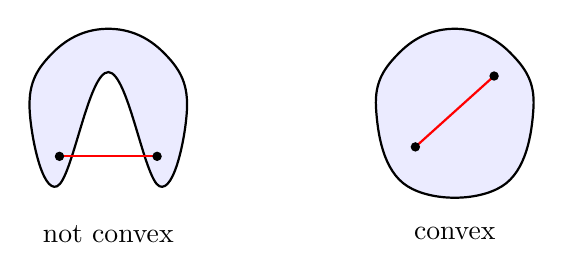
\begin{tikzpicture}[scale=1.0]
		\begin{scope}[shift={(-2.2,0)}]
			\draw [thick, fill=blue!8] plot [smooth cycle, tension=0.7] coordinates {(0, 1) (-0.7, 0.7) (-1, 0) (-0.65, -1) (0, 0.45) (0.65, -1) (1, 0) (0.7, 0.7)};
			\draw [thick, red] (-0.62, -0.62) -- (0.62, -0.62);
			\node at (-0.62,-0.62) [circle, fill, inner sep=1.2pt] {};
			\node at (0.62,-0.62) [circle, fill, inner sep=1.2pt] {};
			\node at (0, -1.6) {not convex};
		\end{scope}
		\begin{scope}[shift={(2.2,0)}]
			\draw [thick, fill=blue!8] plot [smooth cycle, tension=0.7] coordinates {(0, 1) (-0.7, 0.7) (-1, 0) (-0.6, -1) (0.6, -1) (1, 0) (0.7, 0.7)};
			\draw [thick, red] (-0.5, -0.5) -- (0.5, 0.4);
			\node at (-0.5,-0.5) [circle, fill, inner sep=1.2pt] {};
			\node at (0.5,0.4) [circle, fill, inner sep=1.2pt] {};
			\node at (0, -1.6) {convex};
		\end{scope}
	\end{tikzpicture}
\end{center}

\begin{definition}[Convex Function]
	A function $f: S \rightarrow \R$ with $S \subseteq \R^n$ is \vocab{convex} if
	\begin{enumerate}[label=(\roman*)]
		\item its domain $S$ is a convex set, and
		\item for all $x, y \in S$ and $t \in (0, 1)$,
		$$
		f((1 - t)x + ty) \leq (1 - t)f(x) + t f(y).
		$$
	\end{enumerate}
	If the inequality is strict whenever $x \neq y$, we say $f$ is \vocab{strictly convex}. We say $f$ is \vocab{concave} (respectively strictly concave) if $-f$ is convex (respectively strictly convex).
\end{definition}

The second condition is best read geometrically. The right hand side, as $t$ runs over $[0,1]$, traces out the \vocab{chord} joining $(x, f(x))$ to $(y, f(y))$; the left hand side traces out the graph of $f$ between the same two points. So $f$ is convex exactly when its graph lies on or below all of its chords.

\begin{center}
	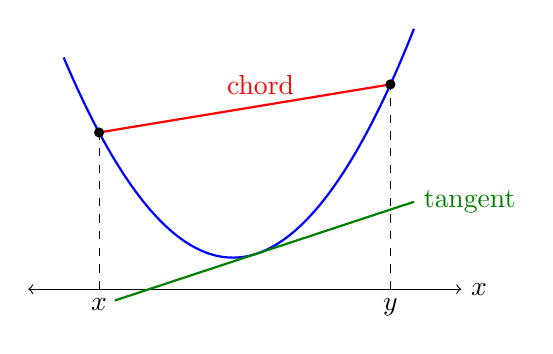
\begin{tikzpicture}[scale=1.0]
		\draw [<->] (-2.6, 0) -- (2.9, 0) node [right] {$x$};
		% the convex function y = 0.55 x^2 + 0.4
		\draw [thick, blue, samples=100, smooth, domain=-2.15:2.3] plot (\x, {0.55*\x*\x + 0.4});
		% chord between x=-1.7 and x=2.0
		\draw [thick, red] (-1.7, 1.98950) -- (2.0, 2.6);
		\node at (-1.7, 1.98950) [circle, fill, inner sep=1.3pt] {};
		\node at (2.0, 2.6) [circle, fill, inner sep=1.3pt] {};
		\draw [dashed] (-1.7, 0) -- (-1.7, 1.98950);
		\draw [dashed] (2.0, 0) -- (2.0, 2.6);
		\node [below] at (-1.7, 0) {$x$};
		\node [below] at (2.0, 0) {$y$};
		% tangent at x = 0.3 : y = 0.55*0.09+0.4 = 0.4495, slope = 1.1*0.3 = 0.33
		\draw [thick, green!50!black] (-1.5, {0.4495 - 0.33*1.8}) -- (2.3, {0.4495 + 0.33*2.0});
		\node [green!50!black, right] at (2.3, {0.4495 + 0.33*2.0}) {tangent};
		\node [red, above left] at (0.9, 2.35) {chord};
	\end{tikzpicture}
\end{center}

We have drawn a tangent line in as well, because it will feature shortly: a convex function also lies \emph{above} all of its tangents.

\begin{example}\leavevmode
	\begin{enumerate}[label=(\roman*)]
		\item $f(x) = x^2$ is strictly convex on $\R$. Indeed,
		$$
		\left[(1-t)x + ty\right]^2 - (1 - t)x^2 - ty^2 = -t(1-t)(x - y)^2 < 0
		$$
		for $t \in (0,1)$ and $x \neq y$, after expanding and collecting terms.
		\item $f(x) = |x|$ is convex, by the triangle inequality, but not strictly so.
		\item $f(x) = 1/x$ on the domain $\{x > 0\}$ is strictly convex.
		\item $f(x) = 1/x$ on $\R \setminus \{0\}$ is \emph{not} convex, for the trivial reason that its domain is not a convex set. This is not mere pedantry: if we tried to patch the definition by setting $f(0) = 0$, the chord from $(-1, -1)$ to $(1, 1)$ would lie below the graph. Condition (i) is doing real work.
	\end{enumerate}
\end{example}

\subsection{Conditions for Convexity}

Checking convexity straight from the definition is unpleasant. If $f$ is differentiable there is a much better test.

\begin{theorem}[First-Order Convexity Condition]\label{vp-thm:foc}
	Let $f$ be differentiable on a convex domain $S$. Then $f$ is convex if and only if
	$$
	f(y) \geq f(x) + (y - x) \cdot \nabla f(x)
	$$
	for all $x, y \in S$.
\end{theorem}
\begin{proof}
	Suppose first that $f$ is convex. Fix $x, y \in S$ and define, for $t \in [0, 1]$,
	$$
	h(t) = (1 - t)f(x) + tf(y) - f((1 - t)x + ty).
	$$
	Convexity says exactly that $h(t) \geq 0$, and clearly $h(0) = 0$. Hence
	$$
	\frac{h(t) - h(0)}{t} \geq 0 \quad \text{for } t \in (0, 1),
	$$
	and letting $t \to 0^+$ gives $h'(0) \geq 0$. On the other hand we may differentiate $h$ directly by the chain rule, giving
	$$
	h'(t) = f(y) - f(x) - (y - x)\cdot \nabla f((1-t)x + ty),
	$$
	so that $h'(0) = f(y) - f(x) - (y - x)\cdot\nabla f(x)$. Combining these gives the inequality.

	Conversely, suppose the inequality holds. Let $z = (1 - t)x + ty$. Applying the inequality twice, at the point $z$,
	\begin{align*}
		f(x) &\geq f(z) + (x - z)\cdot \nabla f(z) = f(z) + t(x - y)\cdot \nabla f(z), \\
		f(y) &\geq f(z) + (y - z)\cdot \nabla f(z) = f(z) - (1-t)(x - y)\cdot \nabla f(z).
	\end{align*}
	Multiplying the first by $(1 - t)$, the second by $t$, and adding, the gradient terms cancel and we are left with
	$$
	(1 - t)f(x) + tf(y) \geq f(z) = f((1-t)x + ty),
	$$
	which is convexity.
\end{proof}

The geometric content is the one we advertised above: $f(x) + (y - x)\cdot\nabla f(x)$ is precisely the tangent plane to the graph of $f$ at $x$, so the condition says that a convex function lies above all of its tangent planes. From this the promised simplification is immediate.

\begin{corollary}
	Any stationary point of a convex function is a global minimum. If $f$ is strictly convex, there is at most one such point.
\end{corollary}
\begin{proof}
	Let $\nabla f(x_0) = 0$. Then \autoref{vp-thm:foc} gives $f(y) \geq f(x_0) + (y - x_0)\cdot 0 = f(x_0)$ for every $y$ in the domain. For the uniqueness statement, if $x_0 \neq x_1$ were two global minima with common value $m$, then strict convexity would give $f(\frac{1}{2}(x_0 + x_1)) < m$, a contradiction.
\end{proof}

By applying \autoref{vp-thm:foc} twice, once at $x$ and once at $y$, and adding the two inequalities, we obtain a symmetric form of the condition:
$$
(y - x)\cdot\left[\nabla f(y) - \nabla f(x)\right] \geq 0.
$$
In one dimension this reads $(y-x)(f'(y) - f'(x)) \geq 0$, which just says $f'$ is non-decreasing. Differentiating one more time gives the criterion that is usually the most convenient of all.

\begin{theorem}[Second-Order Convexity Condition]
	Let $f$ be twice differentiable on a convex domain. Then $f$ is convex if and only if the Hessian $H$ is positive semi-definite at every point (all eigenvalues $\geq 0$). If $H$ is positive definite everywhere, then $f$ is strictly convex.
\end{theorem}
\begin{proof}[Proof (sketch)]
	Put $y = x + h$ in the symmetric first-order condition, so that
	$$
	h \cdot \left[\nabla f(x + h) - \nabla f(x)\right] \geq 0.
	$$
	Taylor expanding the bracket in $h$ using the summation convention, this is
	$$
	h_i\left[h_j \partial_j\partial_i f + O(|h|^2)\right] = h_i H_{ij}h_j + O(|h|^3) \geq 0.
	$$
	Since $h$ is arbitrary and may be taken small, this holds if and only if $h^T H h \geq 0$ for all $h$, i.e.\ $H$ is positive semi-definite.
\end{proof}

\begin{remark}
	The converse of the last sentence is false: $f(x) = x^4$ is strictly convex, but $f''(0) = 0$. So positive definiteness is sufficient but not necessary for strictness.
\end{remark}

\begin{example}
	Let $f(x, y) = 1/(xy)$ on the domain $x, y > 0$. Then
	$$
	H = \frac{1}{xy}\begin{pmatrix}
		2/x^2 & 1/(xy) \\ 1/(xy) & 2/y^2
	\end{pmatrix},
	$$
	so that
	$$
	\det H = \frac{1}{x^2y^2}\left(\frac{4}{x^2y^2} - \frac{1}{x^2y^2}\right) = \frac{3}{x^4 y^4} > 0, \qquad \tr H = \frac{2}{xy}\left(\frac{1}{x^2} + \frac{1}{y^2}\right) > 0.
	$$
	Both eigenvalues are therefore positive and $f$ is strictly convex.

	It is tempting to notice that we only ever used $xy > 0$, and conclude that $f$ is convex on the larger domain $\{xy > 0\}$. This is wrong -- that domain is not connected, let alone convex, and the definition fails at the first hurdle.
\end{example}

\subsection{Inequalities from Convexity}

Convexity is a machine for producing inequalities, and it is worth seeing it run. The starting point is the extension of the defining inequality from two points to many.

\begin{theorem}[Jensen's Inequality]
	Let $f$ be convex, let $x_1, \dots, x_n$ lie in its domain, and let $t_1, \dots, t_n \geq 0$ with $\sum_i t_i = 1$. Then
	$$
	f\left(\sum_{i=1}^n t_i x_i\right) \leq \sum_{i = 1}^n t_i f(x_i).
	$$
\end{theorem}
\begin{proof}
	We induct on $n$. The case $n = 2$ is the definition (the cases $t_i \in \{0,1\}$ being trivial), and $n = 1$ is vacuous. Suppose the result holds for $n - 1$ and let $t_n < 1$ (if $t_n = 1$ there is nothing to prove). Write $s = 1 - t_n = \sum_{i < n} t_i > 0$ and
	$$
	z = \sum_{i = 1}^{n-1}\frac{t_i}{s}x_i,
	$$
	which lies in the domain since the domain is convex and the weights $t_i/s$ sum to $1$. Then $\sum_i t_i x_i = sz + t_n x_n$, so by the $n = 2$ case and then the inductive hypothesis,
	\[
	f\left(\sum_i t_i x_i\right) \leq s f(z) + t_n f(x_n) \leq s \sum_{i<n} \frac{t_i}{s}f(x_i) + t_n f(x_n) = \sum_{i=1}^n t_i f(x_i). \qedhere
	\]
\end{proof}

There is a continuous version too, which is the one that connects to the rest of this article: if $\rho \geq 0$ has $\int \rho = 1$, then $f\left(\int \rho(x) u(x) \dd x\right) \leq \int \rho(x) f(u(x)) \dd x$, proved in the same way by approximating the integral by sums. In probabilistic language this is $f(\EE[U]) \leq \EE[f(U)]$, which is how the reader will have met it in Probability.

\begin{corollary}[AM--GM Inequality]
	For positive reals $a_1, \dots, a_n$,
	$$
	\frac{a_1 + \cdots + a_n}{n} \geq \sqrt[n]{a_1 \cdots a_n}.
	$$
\end{corollary}
\begin{proof}
	The function $f(x) = -\log x$ is convex on $x > 0$, since $f''(x) = 1/x^2 > 0$. Applying Jensen with $t_i = 1/n$ and $x_i = a_i$,
	$$
	-\log\left(\frac{1}{n}\sum_i a_i\right) \leq -\frac{1}{n}\sum_i \log a_i = -\log\left(\prod_i a_i\right)^{1/n}.
	$$
	Multiplying by $-1$ and exponentiating (both $\log$ and $\exp$ being increasing) gives the result.
\end{proof}

The next inequality is really a statement about the Legendre transform in disguise, as we will see in a moment.

\begin{proposition}[Young's Inequality]
	Let $p, q > 1$ with $\frac{1}{p} + \frac{1}{q} = 1$. Then for all $a, b \geq 0$,
	$$
	ab \leq \frac{a^p}{p} + \frac{b^q}{q}.
	$$
\end{proposition}
\begin{proof}
	The case $ab = 0$ is clear, so take $a, b > 0$. Applying Jensen to the convex function $-\log$ with weights $1/p, 1/q$ and points $a^p, b^q$,
	$$
	-\log\left(\frac{a^p}{p} + \frac{b^q}{q}\right) \leq -\frac{1}{p}\log a^p - \frac{1}{q}\log b^q = -\log(ab),
	$$
	and exponentiating gives the claim.
\end{proof}

\begin{corollary}[H\"older's Inequality]
	Let $p, q > 1$ with $\frac 1p + \frac 1q = 1$. Then for reals $u_i, v_i$,
	$$
	\sum_{i=1}^n |u_i v_i| \leq \left(\sum_{i=1}^n |u_i|^p\right)^{1/p}\left(\sum_{i=1}^n |v_i|^q\right)^{1/q}.
	$$
\end{corollary}
\begin{proof}
	Write $U = (\sum_i |u_i|^p)^{1/p}$ and $V = (\sum_i |v_i|^q)^{1/q}$, and assume both are nonzero (otherwise all the $u_i$ or all the $v_i$ vanish and the result is trivial). Apply Young's inequality with $a = |u_i|/U$ and $b = |v_i|/V$ and sum over $i$:
	$$
	\frac{1}{UV}\sum_i |u_iv_i| \leq \frac{1}{p}\frac{\sum_i |u_i|^p}{U^p} + \frac{1}{q}\frac{\sum_i|v_i|^q}{V^q} = \frac{1}{p} + \frac{1}{q} = 1,
	$$
	and multiplying by $UV$ finishes the proof.
\end{proof}

Taking $p = q = 2$ recovers the Cauchy--Schwarz inequality. We will meet a genuinely variational inequality later, when the Rayleigh--Ritz method in \autoref{sec:rayleigh} lets us bound eigenvalues by making guesses.

\subsection{The Legendre Transform}

We now come to a construction which, on first meeting, looks arbitrary, and which turns out to be one of the most useful things in mathematical physics. It appears in thermodynamics (relating energy, free energy and enthalpy), in mechanics (relating the Lagrangian and the Hamiltonian), and in optimisation (as duality).

Here is the motivation. Suppose we have a differentiable function $f(x)$, and for whatever reason we would rather work with the derivative
$$
p = \frac{\dd f}{\dd x}
$$
as our independent variable. In physics $p$ is usually the interesting quantity: for a Lagrangian it is a momentum, for the energy of a gas it is a temperature. The obvious thing to try, $g(p) = f(x(p))$, is a bad idea -- it is not symmetric, it loses information when $f$ has an inflection, and it has no nice properties whatsoever.

What we would \emph{like} is a function $f^*$ with the pleasing reciprocal property
$$
\frac{\dd f^*}{\dd p} = x,
$$
so that if $p$ is conjugate to $x$, then $x$ is conjugate to $p$. In terms of differentials, we have $\dd f = p \dd x$ and we want $\dd f^* = x \dd p$. Since the product rule gives $\dd(xp) = x \dd p + p \dd x$, the choice
$$
f^*(p) = xp - f(x)
$$
does exactly what we want. We take this as our definition, but phrased so as not to require differentiability.

\begin{definition}[Legendre Transform]
	The \vocab{Legendre transform} of a function $f: \R^n \rightarrow \R$ is the function $f^*$ given by
	$$
	f^*(p) = \sup_x \left(p \cdot x - f(x)\right).
	$$
	The domain of $f^*$ is taken to be the set of $p$ for which the supremum is finite. We call $p$ the \vocab{conjugate variable} to $x$.
\end{definition}

In one dimension there is a very clean picture. For a fixed $p$, the quantity $px - f(x)$ is the vertical gap between the line $y = px$ and the graph $y = f(x)$, and $f^*(p)$ is the largest such gap. Equivalently -- and this is the version worth remembering -- draw the tangent line to $f$ of slope $p$; then $-f^*(p)$ is its intercept with the $y$-axis.

\begin{center}
	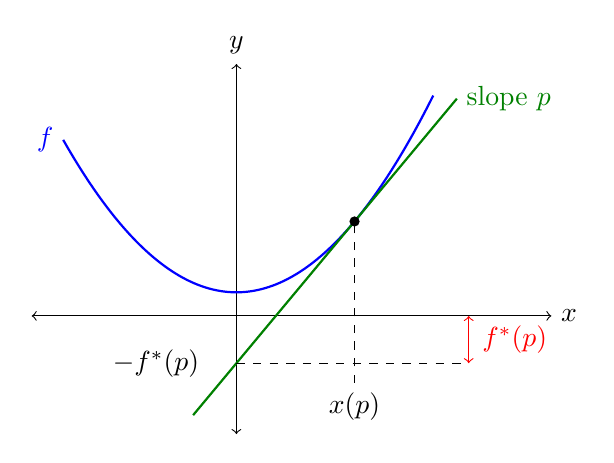
\begin{tikzpicture}[scale=1.0]
		\draw [<->] (-2.6, 0) -- (4.0, 0) node [right] {$x$};
		\draw [<->] (0, -1.5) -- (0, 3.2) node [above] {$y$};
		% f(x) = 0.4 x^2 + 0.3, f'(x) = 0.8x. Take p = 1.2 => x = 1.5, f = 1.2, tangent intercept = f - p x = 1.2 - 1.8 = -0.6
		\draw [thick, blue, samples=100, smooth, domain=-2.2:2.5] plot (\x, {0.4*\x*\x + 0.3});
		\node [blue, left] at (-2.2, {0.4*2.2*2.2 + 0.3}) {$f$};
		% tangent line of slope 1.2 through (1.5, 1.2)
		\draw [thick, green!50!black, domain=-0.55:2.8] plot (\x, {-0.6 + 1.2*\x});
		\node [green!50!black, right] at (2.8, {-0.6 + 1.2*2.8}) {slope $p$};
		% dashed horizontal at y = -0.6, drawn only to the right of the axis
		\draw [dashed] (0, -0.6) -- (2.95, -0.6);
		\node [left] at (-0.35, -0.6) {$-f^*(p)$};
		% tangency point
		\node at (1.5, 1.2) [circle, fill, inner sep=1.3pt] {};
		\draw [dashed] (1.5, -0.85) -- (1.5, 1.2);
		\node [below] at (1.5, -0.85) {$x(p)$};
		% the gap between the intercept and the origin
		\draw [<->, red] (2.95, -0.6) -- (2.95, 0);
		\node [red, right] at (3.0, -0.3) {$f^*(p)$};
	\end{tikzpicture}
\end{center}

Notice that the supremum is finite exactly when the line of slope $p$ can be pushed up against the graph from below, which is why convexity is about to become important.

\begin{proposition}
	If the domain of $f^*$ is non-empty then it is a convex set, and $f^*$ is a convex function -- regardless of whether $f$ is convex.
\end{proposition}
\begin{proof}
	Let $p, q$ lie in the domain of $f^*$ and let $t \in (0,1)$. Then
	\begin{align*}
		f^*((1-t)p + tq) &= \sup_x\left[(1-t)p\cdot x + t q \cdot x - f(x)\right] \\
		&= \sup_x\left[(1-t)\left(p\cdot x - f(x)\right) + t\left(q\cdot x - f(x)\right)\right] \\
		&\leq (1-t)\sup_x\left[p\cdot x - f(x)\right] + t \sup_x\left[q\cdot x - f(x)\right] \\
		&= (1-t)f^*(p) + tf^*(q),
	\end{align*}
	using only that the supremum of a sum is at most the sum of the suprema. In particular the right hand side is finite, so $(1-t)p + tq$ is in the domain, which is therefore convex; and the inequality is exactly convexity of $f^*$.
\end{proof}

In practice, if $f$ is convex and differentiable, we do not compute a supremum at all: we differentiate. The supremum of $p\cdot x - f(x)$ occurs where
$$
\nabla\left(p\cdot x - f(x)\right) = 0 \iff p = \nabla f(x),
$$
and if $f$ is strictly convex then $\nabla f$ is injective, so this can be solved uniquely for $x = x(p)$, giving
$$
f^*(p) = p\cdot x(p) - f(x(p)).
$$

\begin{example}\leavevmode
	\begin{enumerate}[label=(\roman*)]
		\item Let $f(x) = \frac{1}{2}ax^2$ with $a > 0$. Then $p = f'(x) = ax$, so $x = p/a$, and
		$$
		f^*(p) = p\cdot\frac{p}{a} - \frac{1}{2}a\left(\frac{p}{a}\right)^2 = \frac{p^2}{2a}.
		$$
		A parabola transforms to a parabola, with the coefficient inverted. Note that transforming again returns $\frac{1}{2}ax^2$, as we would hope.
		\item Let $f(v) = -\sqrt{1 - v^2}$ on $|v| < 1$ (the lower half of a circle). Then
		$$
		p = f'(v) = \frac{v}{\sqrt{1 - v^2}} \implies v = \frac{p}{\sqrt{1 + p^2}},
		$$
		which exists for all $p \in \R$, and
		$$
		f^*(p) = pv + \sqrt{1 - v^2} = \frac{p^2}{\sqrt{1+p^2}} + \frac{1}{\sqrt{1+p^2}} = \sqrt{1 + p^2}.
		$$
		A circle transforms to a hyperbola. (The reader who has met special relativity may enjoy recognising this.)
		\item Let $f(x) = cx$ for a constant $c$. This is convex but not strictly. Then $px - f(x) = (p - c)x$, which is unbounded above unless $p = c$. So the domain of $f^*$ is the single point $\{c\}$, and $f^*(c) = 0$. A line transforms to a point.
	\end{enumerate}
\end{example}

The last example makes the general phenomenon clear: the Legendre transform trades the `flatness' of a function for the `sharpness' of its transform, and vice versa. It also explains why convexity is exactly the right hypothesis for the following.

\begin{theorem}
	If $f$ is convex and differentiable, then $f^{**} = f$.
\end{theorem}
\begin{proof}
	We have $f^*(p) = p \cdot x(p) - f(x(p))$, where $x(p)$ satisfies $p = \nabla f(x(p))$. Differentiating with respect to $p_i$ and using the product and chain rules,
	\begin{align*}
		\partial_i f^*(p) &= x_i + p_j \partial_i x_j(p) - \partial_i x_j(p)\,\partial_j f(x) \\
		&= x_i + p_j \partial_i x_j(p) - \partial_i x_j(p)\, p_j \\
		&= x_i,
	\end{align*}
	where in the second line we used $p_j = \partial_j f(x)$. So $\nabla f^*(p) = x$: the conjugate variable to $p$ is the original $x$. Therefore
	\[
	f^{**}(x) = \left.\left(x\cdot p - f^*(p)\right)\right|_{p = p(x)} = x\cdot p - \left(p\cdot x - f(x)\right) = f(x). \qedhere
	\]
\end{proof}

Convexity really is needed here. Since $f^{**}$ is a Legendre transform it is automatically convex, so $f^{**} = f$ can only possibly hold for convex $f$. For a non-convex $f$, the double transform $f^{**}$ turns out to be the largest convex function lying below $f$ -- its `convex hull' -- so the transform simply cannot see the non-convex parts.

\begin{remark}
	Young's inequality is now transparent. Take $f(x) = x^p/p$ for $x \geq 0$ and $p > 1$. Then $f^*(b) = \sup_x(bx - x^p/p) = b^q/q$ where $\frac 1p + \frac 1q = 1$, by the usual differentiation. But directly from the definition of a supremum, $f^*(b) \geq ab - f(a)$ for any $a$, which rearranges to $ab \leq a^p/p + b^q/q$. Every Legendre transform gives an inequality in this way, the general statement $p\cdot x \leq f(x) + f^*(p)$ being called \vocab{Fenchel's inequality}.
\end{remark}

\subsection{An Application to Thermodynamics}

The reason a thermodynamics course is full of Legendre transforms is worth a paragraph. Consider a gas of a fixed number of particles in a container. In principle we could write down the equations of motion of all $10^{23}$ particles and solve them, which is not a plan. Instead we describe the gas by a handful of macroscopic quantities: the entropy $S$, volume $V$, pressure $P$ and temperature $T$. The energy is naturally a function
$$
E = E(S, V).
$$
There are two ways to change it: we can do work on the gas by compressing it, contributing $-P\dd V$, or we can heat it, contributing $T \dd S$. So
$$
\dd E = T \dd S - P \dd V,
$$
and comparing with the chain rule,
$$
T = \frac{\partial E}{\partial S}, \qquad P = -\frac{\partial E}{\partial V}.
$$
The trouble is that entropy is not something one can easily hold fixed in a laboratory, whereas temperature is. We would therefore like a function of $T$ and $V$ instead of $S$ and $V$ -- and $T$ is precisely the variable conjugate to $S$. Taking the (negative of the) Legendre transform in $S$ gives the \vocab{Helmholtz free energy}
$$
F(T, V) = \inf_S\left(E(S, V) - TS\right) = E - TS,
$$
where the infimum is at $T = \partial E/\partial S$ as required. Its differential is
$$
\dd F = \dd E - T \dd S - S \dd T = -S\dd T - P \dd V,
$$
so that $S = -\partial F/\partial T$ and $P = -\partial F /\partial V$. This is the whole point: no information has been lost, and we can recover everything by differentiating $F$, which we could not do had we naively substituted $S = S(T, V)$ into $E$.

Transforming instead in $V$ gives the \vocab{enthalpy} $H(S, P) = E + PV$, and transforming in both gives the \vocab{Gibbs free energy} $G(T,P) = E - TS + PV$. The convexity of $E$ in its arguments -- which is a physical statement about the stability of the gas -- is what guarantees these transforms are invertible.

\section{The Euler-Lagrange Equations}

We are now going to move on to deriving some necessary conditions for the extrema of a functional.

\subsection{Deriving the Euler-Lagrange Equations}

We want to extremize the functional \eqref{eq:functional},
$$
	F[y] = \int_{\alpha}^{\beta} f(x, y(x), y'(x)) \dd x,
$$
where we assume that $f$ is given, and that our competing functions have fixed endpoints $y(\alpha) = y_1$ and $y(\beta) = y_2$.

Recall how we found stationary points in $\R^n$: we perturbed our candidate point $a$ by a small displacement, expanded to first order, and demanded that the first-order term vanish for \emph{every} direction of displacement. We shall do precisely the same thing here. The only difference is that a `displacement' is now a whole function, and there are infinitely many directions to worry about.

So suppose $y$ is our candidate extremum, and perturb it to
$$
y \mapsto y + \epsilon \eta(x),
$$
where $\epsilon$ is a small real number and $\eta$ is any (sufficiently smooth) function with
$$
\eta(\alpha) = \eta(\beta) = 0.
$$
The condition on $\eta$ is forced on us: the endpoints of $y$ are fixed, so any admissible competitor must agree with $y$ there.

\begin{center}
	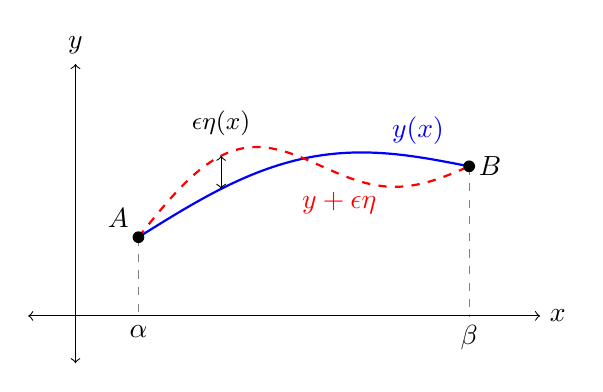
\begin{tikzpicture}[scale=1.0]
		\coordinate (a) at (0.8,1.0);
		\coordinate (b) at (5.0, 1.9);

		% axes
		\draw [<->] (-0.6, 0) -- (5.9, 0) node [right] {$x$};
		\draw [<->] (0, -0.6) -- (0, 3.2) node [above] {$y$};

		% dashed lines to endpoints
		\draw [dashed, gray] (a) -- (0.8, 0) node [black, below] {$\alpha$};
		\draw [dashed, gray] (b) -- (5.0, 0) node [black, below] {$\beta$};

		% the extremal y (blue)
		\draw [thick, blue] plot [smooth, samples=80, domain=0.8:5.0]
			(\x, {1.0 + 0.9*(\x-0.8)/4.2 + 0.55*sin(180*(\x-0.8)/4.2)});
		% the perturbed path y + eps eta (red, dashed)
		\draw [thick, red, dashed] plot [smooth, samples=80, domain=0.8:5.0]
			(\x, {1.0 + 0.9*(\x-0.8)/4.2 + 0.55*sin(180*(\x-0.8)/4.2) + 0.42*sin(360*(\x-0.8)/4.2)});

		\node [blue, above] at (4.35, 2.06) {$y(x)$};
		\node [red, below] at (3.35, 1.70) {$y + \epsilon\eta$};

		% vertical gap arrow at x = 1.85
		\draw [<->, thin] (1.85, 1.614) -- (1.85, 2.034);
		\node [above, font=\small] at (1.85, 2.16) {$\epsilon\eta(x)$};

		% endpoints
		\node at (a) [circle,fill,inner sep=1.5pt] {};
		\node at (b) [circle,fill,inner sep=1.5pt] {};
		\draw (a) node [above left] {$A$};
		\draw (b) node [right] {$B$};
	\end{tikzpicture}
\end{center}

We will compute $F[y + \epsilon \eta]$ and expand in $\epsilon$. To turn the resulting condition into a differential equation, we will need an important lemma.

\begin{lemma}[Fundamental Lemma of Calculus of Variations]\label{lem:fundamental}
	If $g: [\alpha, \beta] \rightarrow \R$ is continuous on $[\alpha, \beta]$ and is such that
	$$
	\int_{\alpha}^{\beta} g(x) \eta(x) \dd x = 0,
	$$
	for all $\eta$ continuous on $[\alpha, \beta]$ with $\eta(\alpha) = \eta(\beta) = 0$, then $g(x) = 0$ for all $x \in [\alpha, \beta]$.
\end{lemma}
\begin{proof}
	Say (for a contradiction) that there exists some $\bar{x} \in (\alpha, \beta)$ such that $g(\bar{x}) \neq 0$. Without loss of generality say $g(\bar{x}) > 0$ (else replace $g$ by $-g$). Then by continuity there exists an interval $[x_1, x_2] \subset (\alpha, \beta)$ containing $\bar{x}$ such that $g(x) > c$ on $[x_1, x_2]$ for some $c > 0$. Then set
	$$
	\eta(x) =
	\begin{cases}
		(x - x_1)(x_2 - x) &\mbox{if } x \in [x_1, x_2], \\
		0 &\mbox{if } x \not \in [x_1, x_2].
	   \end{cases}
	$$
	This $\eta$ is continuous, vanishes at $\alpha$ and $\beta$, is non-negative, and is strictly positive on $(x_1, x_2)$. Since the integrand vanishes off $[x_1, x_2]$, we have
	$$
	   \int_\alpha^\beta g(x) \eta(x) \dd x = \int_{x_1}^{x_2} g(x)\eta(x) \dd x > c \int_{x_1}^{x_2} (x - x_1)(x_2 - x) \dd x = \frac{c(x_2 - x_1)^3}{6} > 0,
	$$
	which is a contradiction. So $g$ vanishes on $(\alpha, \beta)$, and hence by continuity on all of $[\alpha, \beta]$.
\end{proof}

\begin{remark}
	In the proof above, we construct a \emph{bump function} $\eta$. It is possible to make this smoother by taking various powers of the constructed function: replacing $\eta$ by $\left[(x-x_1)(x_2-x)\right]^{k+1}$ on $[x_1, x_2]$ gives a $C^k$ bump. So the lemma remains true if we insist that our test functions be as smooth as we like, which is what we shall actually need.
\end{remark}

The lemma is worth internalising in the following form: the only continuous function which is `invisible' to every test function is the zero function. This is exactly the tool we need to convert an integral condition into a pointwise one.

Now let's return to our computation. We have
\begin{align*}
	F[y + \epsilon \eta] &= \int_{\alpha}^{\beta} f(x, y + \epsilon \eta, y' + \epsilon \eta') \dd x \\
	&= F[y] + \epsilon \int_{\alpha}^{\beta} \left(\frac{\partial f}{\partial y} \eta + \frac{\partial f}{\partial y'} \eta '\right) \dd x + O(\epsilon^2),
\end{align*}
where the partial derivatives are all evaluated along the unperturbed path.
We will return to the $O(\epsilon^2)$ term in \autoref{sec:secondvar}, where it tells us about the \emph{nature} of the stationary point. For now we note that for an extremum we want the first-order term to vanish for \emph{every} admissible $\eta$, that is
$$
\left.\frac{\dd}{\dd \epsilon}F[y + \epsilon \eta]\right|_{\epsilon = 0} = \int_{\alpha}^{\beta}\left(\frac{\partial f}{\partial y}\eta + \frac{\partial f}{\partial y'}\eta'\right)\dd x = 0.
$$
This quantity is called the \vocab{first variation} of $F$ at $y$.

We cannot apply the fundamental lemma to this directly, because the integrand involves $\eta'$ as well as $\eta$. We now make a move which we will return to time and time again in the calculus of variations: we integrate the offending term by parts, so that only $\eta$ appears. This gives
\begin{align*}
	0 &= \int_{\alpha}^{\beta} \left(\frac{\partial f}{\partial y} \eta - \frac{\dd}{\dd x} \left(\frac{\partial f}{\partial y'}\right) \eta\right) \dd x + \cancel{\left[\frac{\partial f}{\partial y'}\eta\right]_{\alpha}^{\beta}} \\
	&= \int_{\alpha}^{\beta} \left(\frac{\partial f}{\partial y} - \frac{\dd}{\dd x} \left(\frac{\partial f}{\partial y'}\right)\right) \eta \dd x,
\end{align*}
the boundary term vanishing precisely because $\eta(\alpha) = \eta(\beta) = 0$.
Applying the fundamental lemma of the calculus of variations, we obtain the following necessary condition for an extremum.

\begin{theorem}[Euler-Lagrange Equation]
	Suppose $y \in C^2_{(\alpha, \beta)}(\R)$ is a function with fixed endpoints that extremizes the functional
	$$
	F[y] = \int_{\alpha}^{\beta} f(x, y(x), y'(x)) \dd x.
	$$
	Then $y$ must satisfy the \vocab{Euler-Lagrange} equation
	\begin{equation}\label{eq:el}
		\frac{\partial f}{\partial y} - \frac{\dd}{\dd x} \left(\frac{\partial f}{\partial y'}\right) = 0. \tag{$\dagger$}
	\end{equation}
\end{theorem}

\begin{notation}
	The LHS of \eqref{eq:el} is denoted by $\displaystyle\frac{\delta F[y]}{\delta y(x)}$ and is the \vocab{functional derivative} of $F$. Writing $\delta y = \epsilon\eta$, the first variation then reads
	$$
	\delta F[y] = \int_\alpha^\beta \frac{\delta F[y]}{\delta y(x)}\,\delta y(x) \dd x,
	$$
	a pleasing analogue of $\dd f = \nabla f \cdot \dd x$ from multivariable calculus. In this language, the Euler--Lagrange equation is simply the statement `$\nabla F = 0$'.
\end{notation}

A few comments are in order before we start solving things.

\begin{remark}\leavevmode
	\begin{enumerate}[label=(\roman*)]
		\item Expanding $\frac{\dd}{\dd x}\left(\partial f/\partial y'\right)$ by the chain rule shows that \eqref{eq:el} is a \emph{second-order} ODE for $y$,
		$$
		\frac{\partial^2 f}{\partial (y')^2}y'' + \frac{\partial^2 f}{\partial y\, \partial y'}y' + \frac{\partial^2 f}{\partial x\, \partial y'} - \frac{\partial f}{\partial y} = 0,
		$$
		to be solved subject to the two conditions $y(\alpha) = y_1$ and $y(\beta) = y_2$. This is a \emph{boundary} value problem rather than an initial value problem, and so, unlike for initial value problems, we get no general guarantee of existence or uniqueness. We will meet examples of both failures.
		\item The Euler--Lagrange equation is a \emph{necessary} condition, not a sufficient one. Exactly like $f'(x) = 0$ in ordinary calculus, it is satisfied by minima, maxima and saddles alike. Determining which we have requires the second variation.
		\item When we write $\partial f/\partial y$, we are treating $x$, $y$ and $y'$ as three \emph{independent} arguments of $f$. This is a genuine source of confusion, and should be carefully distinguished from the total derivative along a path,
		$$
		\frac{\dd}{\dd x} = \frac{\partial}{\partial x} + y'\frac{\partial }{\partial y} + y''\frac{\partial}{\partial y'}.
		$$
		For instance, if $f(x, y, y') = x\left[(y')^2 - y^2\right]$ then $\partial f/\partial x = (y')^2 - y^2$, whereas
		$$
		\frac{\dd f}{\dd x} = (y')^2 - y^2 - 2xyy' + 2xy'y''.
		$$
		These are very different objects.
		\item The boundary term $\left[\eta\,\partial f/\partial y'\right]_\alpha^\beta$ vanished because we fixed the endpoints. It will not always do so, and when it does not we obtain extra `natural' boundary conditions instead; see \autoref{sec:naturalbc}.
	\end{enumerate}
\end{remark}

Before we get to the classical problems, let us do one entirely routine example, just to see the machinery turn over.

\begin{example}
	Let us find the stationary points of
	$$
	F[y] = \int_0^1\left((y')^2 + y^2\right)\dd x, \qquad y(0) = 0, \ y(1) = 1.
	$$
	Here $f = (y')^2 + y^2$, so
	$$
	\frac{\partial f}{\partial y} = 2y, \qquad \frac{\partial f}{\partial y'} = 2y',
	$$
	and the Euler--Lagrange equation \eqref{eq:el} is
	$$
	2y - \frac{\dd}{\dd x}(2y') = 0 \implies y'' = y.
	$$
	The general solution is $y = A\sinh x + B\cosh x$. The condition $y(0) = 0$ gives $B = 0$, and $y(1) = 1$ gives $A = 1/\sinh 1$, so
	$$
	y = \frac{\sinh x}{\sinh 1}.
	$$
	Substituting back (and integrating by parts once) gives the stationary value $F[y] = \coth 1 \approx 1.313$.

	It is worth noticing that we could have got the same answer from the Beltrami identity below, since $f$ has no explicit $x$-dependence: that would give $(y')^2 - y^2 = $ constant, a first-order equation. Either route works, and in general one takes whichever is less painful.
\end{example}

\subsection{First Integrals of the Euler-Lagrange Equations}

Of course, now that we have a necessary condition for extremality, our next concern is solving the Euler-Lagrange equation.
The Euler-Lagrange equations give us a second-order ODE for $y$.
It is sometimes possible to reduce the order of the ODE to get a first-order ODE, a \vocab{first integral}, which is what we will look at in this section.
There are two cases where this happens, and they correspond to the two `missing variables' the integrand might have.

The first case is easy. If $f$ does not explicitly depend on $y$, then $\partial f/\partial y = 0$, and the Euler--Lagrange equation reads
$$
 \frac{\dd}{\dd x} \left(\frac{\partial f}{\partial y'}\right) = 0 \implies \frac{\partial f}{\partial y'} = c,
$$
for some constant $c$. We have integrated the equation once for free, and what remains is a first-order ODE. A variable which does not appear in the integrand (only its derivative does) is called \vocab{cyclic} or \vocab{ignorable}, and every cyclic variable gives us such a conserved quantity. In mechanics these will turn out to be the conserved momenta.

\begin{example}[Geodesics on the Euclidean Plane]
	Consider again the problem of finding geodesics on the Euclidean plane. 

	We want to minimize the functional
	$$
	D[y] = \int_{x_1}^{x_2} \sqrt{1 + (y')^2} \dd x.
	$$
	Using the Euler-Lagrange equations, we have $f(y') = \sqrt{1 + (y')^2}$, so $\partial f/\partial y = 0$, and thus by the result above
	$$
	\frac{y'}{\sqrt{1 + (y')^2}} = c,
	$$
	for some constant $c$. For this to be the case, we must have $y'$ constant, so $y$ is a straight line.
\end{example}

\begin{example}[Geodesics on a Cylinder]
	Consider the cylinder $x^2 + y^2 = a^2$ in $\R^3$, parameterized by an angle $\phi$ and a height $z$. The line element is
	$$
	\dd s^2 = a^2 \dd\phi^2 + \dd z^2,
	$$
	so thinking of $z$ as a function of $\phi$, we wish to extremize
	$$
	F[z] = \int_{\phi_1}^{\phi_2}\sqrt{a^2 + (z')^2}\dd\phi.
	$$
	Now $z$ is cyclic, so
	$$
	\frac{\partial f}{\partial z'} = \frac{z'}{\sqrt{a^2 + (z')^2}} = c,
	$$
	which forces $z'$ to be constant, say $z' = m$, and hence
	$$
	z = m\phi + z_0.
	$$
	This is a \emph{helix}. The special cases are worth noting: $m = 0$ gives a horizontal circle, and letting $m \to \infty$ (that is, treating $\phi$ as a function of $z$ and finding it constant) gives a vertical straight line. All three are what one would draw by wrapping a piece of string around a tube.

	Notice also that between two given points there are \emph{infinitely many} helical geodesics -- one for each number of times we wind around the cylinder -- of which only one is shortest. Once again, the Euler--Lagrange equation cannot tell them apart.
\end{example}


\begin{example}[Geodesics on the Sphere]
	Consider the sphere embedded in three-dimensional Euclidean space, $S^2 \subset \R^3$, and two points $A$ and $B$ on the sphere. We want to find the shortest path between $A$ and $B$.

	\begin{center}
		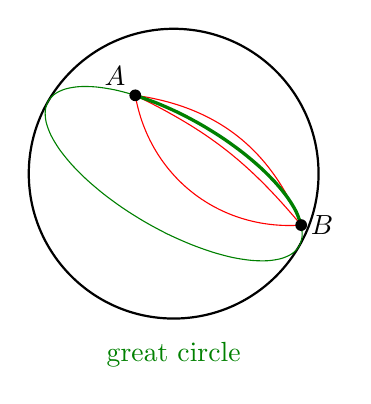
\begin{tikzpicture}[scale=1.15]
			% The sphere outline
			\draw [thick] (0, 0) circle (1.6);

			% Two points on the sphere, lying on the great circle below
			\coordinate (a) at (-0.424, 0.865);
			\coordinate (b) at (1.408, -0.568);

			% The great circle through A and B, as a projected ellipse
			\draw [thin, green!50!black] plot [smooth cycle] coordinates {(1.386,-0.800) (1.418,-0.695) (1.408,-0.568) (1.355,-0.424) (1.261,-0.268) (1.128,-0.103) (0.961,0.065) (0.765,0.231) (0.546,0.390) (0.310,0.537) (0.065,0.668) (-0.183,0.778) (-0.424,0.865) (-0.653,0.926) (-0.862,0.958) (-1.045,0.961) (-1.196,0.935) (-1.311,0.881) (-1.386,0.800) (-1.418,0.695) (-1.408,0.568) (-1.355,0.424) (-1.261,0.268) (-1.128,0.103) (-0.961,-0.065) (-0.765,-0.231) (-0.546,-0.390) (-0.310,-0.537) (-0.065,-0.668) (0.183,-0.778) (0.424,-0.865) (0.653,-0.926) (0.862,-0.958) (1.045,-0.961) (1.196,-0.935) (1.311,-0.881)};

			% Competing (non-geodesic) paths
			\draw [red] (a) to [bend right=42] (b);
			\draw [red] (a) to [bend left=30] (b);
			\draw [red] (a) to [bend left=12] (b);

			% The minor arc from A to B, lying exactly on the great circle
			\draw [very thick, green!50!black] plot [smooth] coordinates {(1.408,-0.568) (1.355,-0.424) (1.261,-0.268) (1.128,-0.103) (0.961,0.065) (0.765,0.231) (0.546,0.390) (0.310,0.537) (0.065,0.668) (-0.183,0.778) (-0.424,0.865)};

			% Points
			\node at (b) [circle,fill,inner sep=1.5pt] {};
			\draw (b) node [right] {$B$};
			\node at (a) [circle,fill,inner sep=1.5pt] {};
			\draw (a) node [above left] {$A$};

			\node [green!50!black, below] at (0, -1.75) {great circle};
		\end{tikzpicture}
	\end{center}

	We first parameterize the sphere, with
	\begin{align*}
		x &= \sin \theta \sin \phi, \\
		y &= \sin \theta \cos \phi, \\
		z &= \cos \theta,
	\end{align*}
	where $0 < \theta \leq \pi$ and $0 \leq \phi \leq 2 \pi$. Then to find lengths of paths on the sphere, we use the line element
	$$
	\dd s^2 = \dd x^2 + \dd y^2 + \dd z^2 = \dd \theta^2 + \sin^2 \theta \dd \phi^2.
	$$
	Now we can parameterize a curve by thinking of $\phi$ as a function of $\theta$. Then we have
	$$
	\dd s = \sqrt{1 + \sin^2 \theta \cdot (\phi')^2} \dd \theta.
	$$
	Thus the functional we want to extremize is
	$$
	F[\phi] = \int_{\alpha}^{\beta} \sqrt{1 + \sin^2 \theta \cdot (\phi')^2} \dd \theta.
	$$
	We note here that $\partial f/ \partial \theta = 0$, so using the result we obtained above, $\partial f/\partial \phi' = \kappa$, for some constant $\kappa$. That is,
	$$
\frac{\sin^2 \theta \cdot \phi'}{\sqrt{1 + \sin^2 \theta \cdot (\phi')^2}} = \kappa.
	$$
	Squaring this and solving for $(\phi')^2$, we get\footnote{There is a sign ambiguity, corresponding to going either forwards or backwards around the sphere.}
	$$
	(\phi')^2 = \frac{\kappa^2}{\sin^2 \theta \left(\sin^2 \theta - \kappa^2\right)} \implies \phi = \pm \int \frac{\kappa \dd \theta}{\sin \theta \sqrt{\sin^2 \theta - \kappa^2}}.
	$$
	This looks unpleasant, but yields to the substitution $u = \cot\theta$, for which $\dd u = -\csc^2\theta \dd\theta$. Writing $\sin^2\theta - \kappa^2 = \sin^2\theta\left[(1 - \kappa^2) - \kappa^2 u^2\right]$ after dividing through by $\sin^2\theta$ and using $\csc^2\theta = 1 + u^2$, the integral becomes
	$$
	\phi - \phi_0 = \mp\int \frac{\kappa \dd u}{\sqrt{(1 - \kappa^2) - \kappa^2 u^2}} = \mp \arcsin\left(\frac{\kappa u}{\sqrt{1 - \kappa^2}}\right),
	$$
	for some constant $\phi_0$. Rearranging, and absorbing the sign into $\phi_0$,
	$$
	\cot\theta = \frac{\sqrt{1 - \kappa^2}}{\kappa}\sin(\phi - \phi_0).
	$$
	To see what this is, multiply through by $\sin\theta$ and expand the sine:
	$$
	\cos\theta = \frac{\sqrt{1 - \kappa^2}}{\kappa}\left(\sin\theta\cos\phi\cos\phi_0 - \sin\theta\sin\phi \sin\phi_0\right).
	$$
	In terms of our Cartesian coordinates this says $z = c_1 y + c_2 x$ for constants $c_1, c_2$, which is the equation of a plane through the origin. So the geodesic lies on the intersection of the sphere with a plane through its centre: it is an arc of a \vocab{great circle}, as we expected.

	Note that the Euler--Lagrange equation cannot distinguish the \emph{minor} arc from the \emph{major} arc -- both are stationary. We will resolve this in \autoref{sec:secondvar} using the second variation, where we find that the major arc fails to be a minimum. Note also that if $A$ and $B$ are antipodal, there are infinitely many geodesics between them, which is our promised failure of uniqueness.
\end{example}

The second case is subtler, and considerably more useful. Consider, for general $f(x, y, y')$, the quantity $f - y' \partial f/\partial y'$. Differentiating along a path with the total derivative,
\begin{align*}
	\frac{\dd}{\dd x} \left(f - y' \frac{\partial f}{\partial y'}\right) &= \frac{\partial f}{\partial x} + y' \frac{\partial f}{\partial y} + \cancel{y'' \frac{\partial f}{\partial y'}} -\cancel{ y'' \frac{\partial f}{\partial y'}} - y' \frac{\dd}{\dd x}\left(\frac{\partial f}{\partial y'}\right) \\
	&= y' \left(\frac{\partial f}{\partial y} - \frac{\dd}{\dd x} \frac{\partial f}{\partial y'}\right) + \frac{\partial f}{\partial x} \\
	&= \frac{\partial f}{\partial x},
\end{align*}
where in the last line we used the Euler-Lagrange equations to kill the bracket. So if $f$ does not depend explicitly on $x$, we obtain another first integral.

\begin{proposition}[Beltrami Identity]\label{prop:beltrami}
	If $f = f(y, y')$ has no explicit $x$-dependence, then along any solution of the Euler--Lagrange equation
	$$
	f - y' \frac{\partial f}{\partial y'} = c
	$$
	for some constant $c$.
\end{proposition}

This is a genuinely powerful trick: a great many of the classical problems have integrands with no explicit $x$, and the Beltrami identity reduces the second-order equation to a first-order separable one in one move. The reader should note that it also has a physical meaning which we will uncover in \autoref{sec:hamilton}: if $x$ is time, then $y'\partial f/\partial y' - f$ is exactly the \emph{energy}, and its constancy is conservation of energy.

\begin{example}[The Brachistochrone]
	Consider again the problem of finding the shape of a wire which gives the shortest travel time for a particle sliding along it, beginning at rest.
	
	We want to minimize the functional
	$$
	T[y] = \frac{1}{\sqrt{2g}} \int_0^{x_2} \frac{\sqrt{1 + (y')^2}}{\sqrt{-y}} \dd x,
	$$
	subject to $y(x_1) =y_1$ and $y(x_2) = y_2$. Here, $f$ does not depend on $x$ and thus we can apply the result above to get 
	$$
		\frac{\sqrt{1 + (y')^2}}{\sqrt{-y}} - y' \frac{y'}{\sqrt{1 + (y')^2} \sqrt{-y}} = \kappa,
	$$
	for some constant $\kappa$. We can solve this differential equation by simplifying to get
	$$
	\frac{1}{\sqrt{1 + (y')^2}} = \kappa \sqrt{-y},
	$$
	and then we can separate variables to get
	$$
	x = \pm \kappa \int \frac{\sqrt{-y}}{\sqrt{1 + \kappa^2 y}} \dd y.
	$$
	The substitution $y = -\frac{1}{\kappa^2} \sin^2 \frac{\theta}{2}$ then gives (after some algebra)
	$$
	x = \pm \frac{1}{2\kappa^2}(\theta - \sin \theta) + C,
	$$
	for some constant $C$. Our particle starts at the origin at $\theta = 0$, so $C = 0$; taking the positive root and writing $a = 1/(2\kappa^2)$, the solution is
	$$
	\left\{\begin{array}{l}
		x= a\left(\theta - \sin\theta\right), \\
		y= -a\left(1 - \cos\theta\right).
		\end{array}\right.
	$$
	This is the parameterized equation of a \vocab{cycloid}: the curve traced by a point on the rim of a wheel of radius $a$ rolling (here, on the underside of the $x$-axis) with constant speed. The constant $a$, and the final value of $\theta$, are fixed by requiring the curve to pass through $B$.

	\begin{center}
		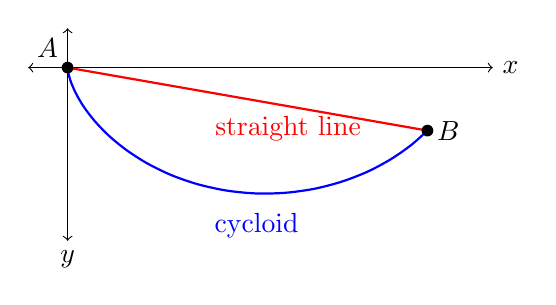
\begin{tikzpicture}[scale=1.0]
			% axes
			\draw [<->] (-0.5, 0) -- (5.4, 0) node [right] {$x$};
			\draw [<->] (0, 0.5) -- (0, -2.2) node [below] {$y$};

			% straight line from A to B
			\draw [thick, red] (0,0) -- (4.570,-0.800);
			\node [red, below] at (2.8, -0.50) {straight line};

			% the cycloid
			\draw [thick, blue] plot [smooth] coordinates {(0.000,-0.000) (0.002,-0.022) (0.014,-0.087) (0.046,-0.192) (0.107,-0.330) (0.203,-0.494) (0.341,-0.675) (0.522,-0.863) (0.747,-1.047) (1.014,-1.218) (1.319,-1.366) (1.655,-1.482) (2.015,-1.561) (2.388,-1.598) (2.764,-1.590) (3.134,-1.539) (3.486,-1.447) (3.813,-1.320) (4.106,-1.163) (4.359,-0.987) (4.570,-0.800)};
			\node [blue, below] at (2.4, -1.72) {cycloid};

			% endpoints
			\node at (0,0) [circle,fill,inner sep=1.5pt] {};
			\node at (4.570,-0.800) [circle,fill,inner sep=1.5pt] {};
			\draw (0,0) node [above left] {$A$};
			\draw (4.570,-0.800) node [right] {$B$};
		\end{tikzpicture}
	\end{center}

	The shape is worth a moment's thought. The optimal wire dives steeply at first, even though this takes the particle \emph{below} $B$ and forces it to climb back up at the end. The reason is that the early plunge buys speed, and the extra speed is worth more than the extra distance. This is the sort of answer one would be unlikely to guess.
\end{example}


\subsection{Fermat's Principle}\label{sec:fermat}

We can now look properly at the first variational principle in this course, which describes the motion of light.

\begin{law}[Fermat's Principle]
Light travels along the path between two points which requires the least time.
\end{law}

Suppose we had a ray with path $y = y(x)$, and suppose the speed of light at $(x, y)$ is $c(x, y)$. Then we want to extremize the functional
$$
F[y] = \int \frac{1}{c} \dd s = \int_{\alpha}^{\beta} \frac{\sqrt{1 + (y')^2}}{c(x, y)} \dd x.
$$
If we assume that $c$ depends only on $x$ -- so the medium is stratified into vertical layers -- then we have $\partial f /\partial y = 0$, and we can use the results of the previous section to obtain
$$
\frac{\partial f}{\partial y'} = \frac{y'}{\sqrt{1 + (y')^2}\, c(x)} = k
$$
for some constant $k$.

Now let $\theta$ be the angle the ray makes with the $x$-axis, so that $\tan\theta = y'$ and hence
$$
\frac{y'}{\sqrt{1 + (y')^2}} = \frac{\tan\theta}{\sec\theta} = \sin\theta.
$$
Our first integral therefore says that $\sin\theta / c(x)$ is constant along the ray:
$$
\frac{\sin \theta_1}{c(x_1)} = \frac{\sin \theta}{c(x)},
$$
which is exactly \vocab{Snell's law} in optics.

\begin{center}
	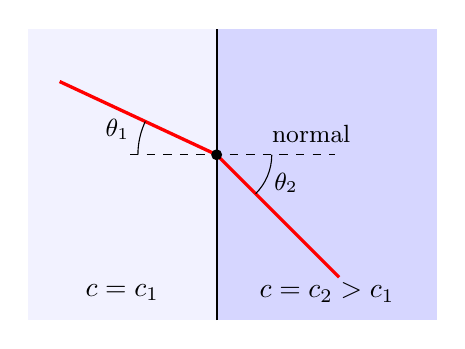
\begin{tikzpicture}[scale=1.0]
		% two media separated by a vertical interface at x = 2.4
		\fill [blue!5] (0, -2.1) rectangle (2.4, 1.6);
		\fill [blue!16] (2.4, -2.1) rectangle (5.2, 1.6);
		\draw [thick] (2.4, -2.1) -- (2.4, 1.6);

		% normal to the interface
		\draw [dashed] (1.3, 0) -- (3.9, 0);
		\node [above, font=\small] at (3.6, 0.03) {normal};

		% incoming ray at 25 degrees to the normal, outgoing at 45 degrees
		\draw [very thick, red] (0.406, 0.930) -- (2.4, 0);
		\draw [very thick, red] (2.4, 0) -- (3.956, -1.556);

		% angle arcs (measured from the horizontal normal)
		\draw [thin] (1.40, 0) arc (180:155:1.00);
		\node [font=\small] at (1.14, 0.32) {$\theta_1$};
		\draw [thin] (3.10, 0) arc (0:-45:0.70);
		\node [font=\small] at (3.281, -0.356) {$\theta_2$};

		\node at (1.2, -1.75) {$c = c_1$};
		\node at (3.8, -1.75) {$c = c_2 > c_1$};

		\node at (2.4, 0) [circle, fill, inner sep=1.4pt] {};
	\end{tikzpicture}
\end{center}

In the picture we have taken $c$ to jump from $c_1$ to a larger value $c_2$ at an interface. Snell's law then reads $\sin\theta_1/c_1 = \sin\theta_2/c_2$, so $\theta_2 > \theta_1$: the ray bends away from the normal on entering the faster medium. This is the familiar refraction of light on passing from glass into air. More generally, in a medium where $c$ increases with $x$, the angle $\theta$ increases too, and the ray curves -- which is exactly the mechanism behind mirages, where hot air near the ground has a higher $c$.

\section{Extensions of the Euler-Lagrange Equations}

We are now going to see how the Euler-Lagrange equations can be used in settings that are not just unconstrained functional extremization of a single function of a single variable. In each case the derivation is the same three-step dance -- perturb, integrate by parts, apply the fundamental lemma -- and only the bookkeeping changes.

\subsection{Several Dependent Variables}\label{sec:multidep}

Suppose that instead of a single function $y$, we have a vector of them,
$$
\vv{y}(x) = \left(y_1(x), \dots, y_n(x)\right),
$$
and we wish to extremize
$$
F[\vv{y}] = \int_\alpha^\beta f\left(x, y_1, \dots, y_n, y_1', \dots, y_n'\right)\dd x,
$$
over functions with all the $y_i$ fixed at the endpoints. This is the situation for, say, a particle moving in three dimensions, where $\vv{y}$ is its position.

The derivation goes through unchanged. Perturb by $\vv{y} \mapsto \vv{y} + \epsilon \bm{\eta}$ where $\bm\eta = (\eta_1, \dots, \eta_n)$ vanishes at both endpoints, expand, and integrate each term by parts:
$$
F[\vv{y} + \epsilon\bm\eta] - F[\vv{y}] = \epsilon\int_\alpha^\beta \sum_{i=1}^n \eta_i \left(\frac{\partial f}{\partial y_i} - \frac{\dd}{\dd x}\frac{\partial f}{\partial y_i'}\right)\dd x + O(\epsilon^2).
$$
Now here is the one new idea. The $\eta_i$ are independent of one another, so we are free to take $\eta_j \equiv 0$ for all $j \neq i$, leaving a single term to which the fundamental lemma applies. Doing this for each $i$ in turn gives:

\begin{theorem}[Euler--Lagrange Equations, Several Dependent Variables]
	A stationary point of $F[\vv y]$ satisfies
	$$
	\frac{\partial f}{\partial y_i} - \frac{\dd}{\dd x}\left(\frac{\partial f}{\partial y_i'}\right) = 0, \qquad i = 1, \dots, n.
	$$
\end{theorem}

This is a coupled system of $n$ second-order ODEs. Both first integrals survive: if $f$ has no explicit dependence on some particular $y_j$, then $\partial f/\partial y_j' $ is constant; and if $f$ has no explicit dependence on $x$, then
$$
f - \sum_{i=1}^n y_i' \frac{\partial f}{\partial y_i'} = \text{constant},
$$
by exactly the computation we did for \autoref{prop:beltrami}.

\begin{example}[Geodesics, Parameterized Properly]
	Our earlier treatment of geodesics in the plane had a defect: by writing $y$ as a function of $x$, we quietly assumed that the shortest curve never doubles back. We can avoid this by parameterizing the curve as $\vv{r}(t) = (x(t), y(t))$ for $t \in [0,1]$, with $\vv{r}(0) = A$ and $\vv{r}(1) = B$, and minimising
	$$
	L[x, y] = \int_0^1 \sqrt{\dot x^2 + \dot y^2}\dd t.
	$$
	Neither $x$ nor $y$ appears explicitly, so both are cyclic and we get two first integrals:
	$$
	\frac{\dot x}{\sqrt{\dot x^2 + \dot y^2}} = c, \qquad \frac{\dot y}{\sqrt{\dot x^2 + \dot y^2}} = s.
	$$
	These constants are not independent: squaring and adding gives $c^2 + s^2 = 1$, so we may write $c = \cos\vartheta$ and $s = \sin\vartheta$. Then both equations reduce to $\dot x \sin\vartheta = \dot y \cos\vartheta$, which integrates to
	$$
	y\cos\vartheta = x \sin\vartheta + A,
	$$
	a straight line of gradient $\tan\vartheta$. Note how the redundancy in the parameterization showed up as a redundancy in the equations -- this is characteristic of problems with a reparameterization symmetry.
\end{example}

\subsection{Several Independent Variables}

Now we go the other way, and let our unknown be a function of several variables. Suppose $\phi = \phi(x, y, z)$ on a domain $\mathcal{D}\subseteq \R^3$, and consider
$$
F[\phi] = \iiint_{\mathcal{D}} f\left(x, y, z, \phi, \phi_x, \phi_y, \phi_z\right)\dd x \dd y \dd z,
$$
where $\phi_{x_i} = \partial\phi/\partial x_i$, and where $\phi$ is prescribed on the boundary $\partial \mathcal{D}$.

Perturb by $\phi \mapsto \phi + \epsilon \eta$ with $\eta = 0$ on $\partial\mathcal D$. The first-order term is
$$
\epsilon\iiint_{\mathcal D}\left(\eta \frac{\partial f}{\partial \phi} + \eta_x \frac{\partial f}{\partial \phi_x} + \eta_y \frac{\partial f}{\partial \phi_y} + \eta_z \frac{\partial f}{\partial \phi_z}\right)\dd V.
$$
The role of integration by parts is now played by the divergence theorem. Writing
$$
\vv{w} = \left(\frac{\partial f}{\partial \phi_x}, \frac{\partial f}{\partial \phi_y}, \frac{\partial f}{\partial \phi_z}\right),
$$
the last three terms are $\nabla \eta \cdot \vv{w} = \nabla\cdot(\eta \vv w) - \eta\, \nabla\cdot \vv{w}$, and the divergence term integrates to $\oint_{\partial \mathcal D}\eta\, \vv{w}\cdot \dd \vv{S} = 0$ since $\eta$ vanishes on the boundary. So we are left with
$$
\epsilon\iiint_{\mathcal D}\eta\left(\frac{\partial f}{\partial \phi} - \nabla\cdot\vv{w}\right)\dd V = 0,
$$
and a version of the fundamental lemma in several variables (proved by exactly the same bump-function argument, in a small ball rather than an interval) gives the following.

\begin{theorem}[Euler--Lagrange Equation, Several Independent Variables]
	A stationary point of $F[\phi]$ satisfies
	$$
	\frac{\partial f}{\partial \phi} - \nabla\cdot\left(\frac{\partial f}{\partial \phi_x}, \frac{\partial f}{\partial \phi_y}, \frac{\partial f}{\partial \phi_z}\right) = 0,
	$$
	or in suffix notation with the summation convention,
	$$
	\frac{\partial f}{\partial \phi} - \partial_i\left(\frac{\partial f}{\partial (\partial_i \phi)}\right) = 0.
	$$
\end{theorem}

Note that this is now a \emph{partial} differential equation for $\phi$. Nothing about the derivation used $n = 3$, and the same statement holds in any number of independent variables.

\begin{example}[Laplace's Equation]
	Consider the `energy' functional
	$$
	F[\phi] = \iint_{\mathcal D \subseteq \R^2}\frac{1}{2}\left(\phi_x^2 + \phi_y^2\right)\dd x \dd y = \iint_{\mathcal D}\frac 12 |\nabla \phi|^2 \dd A,
	$$
	which is (up to constants) the electrostatic energy of a potential $\phi$, or the elastic energy of a stretched membrane with height $\phi$. Here $\partial f/\partial\phi = 0$ and $\partial f/\partial \phi_x = \phi_x$, $\partial f/\partial \phi_y = \phi_y$, so the Euler--Lagrange equation is
	$$
	\phi_{xx} + \phi_{yy} = 0,
	$$
	which is Laplace's equation. So harmonic functions are exactly the stationary points of the Dirichlet energy -- a fact known as \emph{Dirichlet's principle}, and one of the classical bridges between the calculus of variations and PDE theory. The reader will recognise the equation, and the tools for solving it, from the Laplace's equation chapter of my Methods notes.
\end{example}

\subsection{Higher Derivatives}

Occasionally our integrand involves higher derivatives of $y$:
$$
F[y] = \int_\alpha^\beta f\left(x, y, y', \dots, y^{(n)}\right)\dd x.
$$
Now we need to fix more data at the endpoints -- specifically $y, y', \dots, y^{(n-1)}$ -- and correspondingly our variations $\eta$ must satisfy $\eta^{(k)}(\alpha) = \eta^{(k)}(\beta) = 0$ for $k = 0, \dots, n-1$. The first variation is
$$
\epsilon\int_\alpha^\beta\left(\frac{\partial f}{\partial y}\eta + \frac{\partial f}{\partial y'}\eta' + \cdots + \frac{\partial f}{\partial y^{(n)}}\eta^{(n)}\right)\dd x,
$$
and we now integrate the $\eta^{(k)}$ term by parts $k$ times. Every boundary term produced involves some $\eta^{(j)}$ with $j \leq n-1$ evaluated at an endpoint, so every one of them vanishes. Each integration by parts contributes a sign, and applying the fundamental lemma gives
$$
\frac{\partial f}{\partial y} - \frac{\dd}{\dd x}\frac{\partial f}{\partial y'} + \frac{\dd^2}{\dd x^2}\frac{\partial f}{\partial y''} - \cdots + (-1)^n \frac{\dd^n}{\dd x^n}\frac{\partial f}{\partial y^{(n)}} = 0.
$$

\begin{example}
	Let us extremize
	$$
	F[y] = \int_0^1 (y'')^2 \dd x, \qquad y(0) = y'(0) = 0, \quad y(1) = 0, \ y'(1) = 1.
	$$
	Here $\partial f/\partial y = \partial f/\partial y' = 0$ and $\partial f/\partial y'' = 2y''$, so the equation is
	$$
	\frac{\dd^2}{\dd x^2}\left(2y''\right) = 0 \implies y'''' = 0,
	$$
	so $y$ is a cubic. Imposing $y(0) = y'(0) = 0$ kills the constant and linear terms, so $y = ax^3 + bx^2$; then $y(1) = 0$ gives $a + b = 0$ and $y'(1) = 1$ gives $3a + 2b = 1$, whence $a = 1, b = -1$:
	$$
	y_0 = x^3 - x^2.
	$$

	In fact we can show that this is an \emph{absolute} minimum, and it is instructive to see how, since the argument does not involve second variations at all. Let $\eta$ be \emph{any} function (not necessarily small) with $\eta = \eta' = 0$ at both endpoints, and not identically zero. Then
	$$
	F[y_0 + \eta] - F[y_0] = \int_0^1(\eta'')^2\dd x + 2\int_0^1 y_0''\eta''\dd x.
	$$
	The first integral is strictly positive. For the second, $y_0'' = 6x - 2$, so integrating by parts twice,
	$$
	2\int_0^1 (6x - 2)\eta''\dd x = 2\left[(6x-2)\eta'\right]_0^1 - 12\int_0^1 \eta'\dd x = 2\left[(6x-2)\eta'\right]_0^1 - 12\left[\eta\right]_0^1 = 0,
	$$
	since $\eta$ and $\eta'$ vanish at both endpoints. Hence $F[y_0 + \eta] > F[y_0]$ for every admissible $\eta \neq 0$, and $y_0$ is the unique global minimiser. When such an argument is available it is much less work than computing second variations.
\end{example}

\subsection{Variable Endpoints and Natural Boundary Conditions}\label{sec:naturalbc}

Throughout the derivation of the Euler--Lagrange equation we quietly used the fixed endpoints twice: once to argue that $\eta$ must vanish there, and once to discard the boundary term
$$
\left[\eta \frac{\partial f}{\partial y'}\right]_\alpha^\beta.
$$
What if one of the endpoints is not fixed? Suppose, for instance, that $y(\alpha) = y_1$ is prescribed, but the value $y(\beta)$ is free -- the curve must end somewhere on the vertical line $x = \beta$, but we do not care where. This is the situation of a bead threaded on a rail.

\begin{center}
	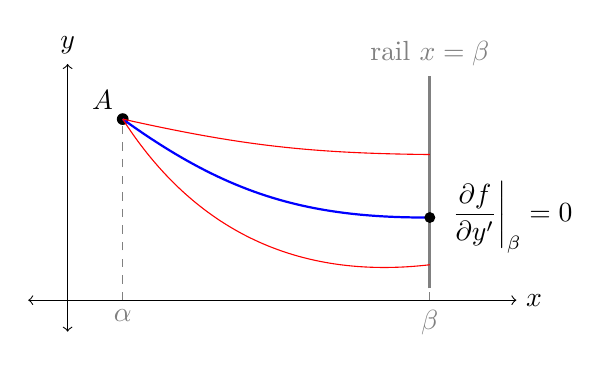
\begin{tikzpicture}[scale=1.0]
		% axes
		\draw [<->] (-0.5, 0) -- (5.7, 0) node [right] {$x$};
		\draw [<->] (0, -0.4) -- (0, 3.0) node [above] {$y$};

		% the rail at x = 4.6
		\draw [very thick, gray] (4.6, 0.15) -- (4.6, 2.85);
		\node [gray, above] at (4.6, 2.85) {rail $x = \beta$};

		% fixed start
		\coordinate (a) at (0.7, 2.3);
		\node at (a) [circle,fill,inner sep=1.5pt] {};
		\node [above left] at (a) {$A$};
		\draw [dashed, gray] (0.7, 0) node [below] {$\alpha$} -- (a);
		\draw [dashed, gray] (4.6, 0) node [below] {$\beta$} -- (4.6, 0.15);

		% candidate curves ending at different heights on the rail
		\draw [thick, blue] (a) to [bend right=18] (4.6, 1.05);
		\draw [thin, red] (a) to [bend right=32] (4.6, 0.45);
		\draw [thin, red] (a) to [bend right=6] (4.6, 1.85);
		\node at (4.6, 1.05) [circle,fill,inner sep=1.4pt] {};
		\node [right] at (4.72, 1.05) {$\displaystyle\left.\frac{\partial f}{\partial y'}\right|_\beta = 0$};
	\end{tikzpicture}
\end{center}

Repeating the derivation, the first variation is
$$
\epsilon\int_\alpha^\beta \eta \left(\frac{\partial f}{\partial y} - \frac{\dd}{\dd x}\frac{\partial f}{\partial y'}\right)\dd x + \epsilon\left[\eta \frac{\partial f}{\partial y'}\right]_\alpha^\beta,
$$
and we still have $\eta(\alpha) = 0$, so the boundary term is just $\epsilon\, \eta(\beta)\left.\partial f/\partial y'\right|_\beta$.

Now we argue in two stages. First restrict to those $\eta$ which \emph{do} vanish at $\beta$; for these the boundary term drops out and we conclude as before that $y$ satisfies the Euler--Lagrange equation. But then, for a general $\eta$, the integral term vanishes automatically, and we are left with
$$
\eta(\beta)\left.\frac{\partial f}{\partial y'}\right|_{x = \beta} = 0.
$$
Since $\eta(\beta)$ is now arbitrary, we must have

\begin{theorem}[Natural Boundary Condition]
	If $y$ extremizes $F[y] = \int_\alpha^\beta f(x, y, y')\dd x$ with $y(\alpha)$ fixed and $y(\beta)$ free, then $y$ satisfies the Euler--Lagrange equation together with the \vocab{natural boundary condition}
	$$
	\left.\frac{\partial f}{\partial y'}\right|_{x = \beta} = 0.
	$$
\end{theorem}

The name is apt: we did not impose this condition, the variational problem produced it for us. Notice that the count works out -- we lost one boundary condition by freeing the endpoint, and gained exactly one back.

\begin{example}
	Consider the shortest path from a fixed point $A = (0, y_1)$ to the line $x = \beta$. Here $f = \sqrt{1 + (y')^2}$, and we already know the Euler--Lagrange equation forces a straight line. The natural boundary condition is
	$$
	\left.\frac{y'}{\sqrt{1 + (y')^2}}\right|_{\beta} = 0 \implies y'(\beta) = 0.
	$$
	Since $y$ is a straight line, $y' \equiv 0$: the shortest path is horizontal, meeting the rail at right angles. This is obvious geometrically, which is a good sanity check on the machinery.
\end{example}

\begin{example}
	Here is a less obvious one. Consider
	$$
	F[y] = \int_0^1\left((y')^2 + y^2 \right)\dd x, \qquad y(0) = 1, \quad y(1) \text{ free}.
	$$
	As we computed earlier, the Euler--Lagrange equation is $y'' = y$, so $y = A\sinh x + B\cosh x$, and $y(0) = 1$ gives $B = 1$. The natural boundary condition is
	$$
	\left.2y'\right|_{x = 1} = 0 \implies y'(1) = 0,
	$$
	so $A\cosh 1 + \sinh 1 = 0$, giving $A = -\tanh 1$ and
	$$
	y = \cosh x - \tanh 1 \sinh x = \frac{\cosh(1 - x)}{\cosh 1}.
	$$
	Notice that the free endpoint has arranged itself so that the curve arrives with zero gradient. Had we instead fixed $y(1) = 0$, we would have obtained a quite different function.
\end{example}

If \emph{both} endpoints are free, the argument runs the same way and we obtain two natural conditions, $\left.\partial f/\partial y'\right|_\alpha = \left.\partial f/\partial y'\right|_\beta = 0$. More generally, a mixture is possible: one endpoint fixed and one free, or a `spring' term added to the functional at the endpoint, in which case the natural condition becomes a Robin-type condition rather than a Neumann one. The general principle is simply that the boundary term in the first variation must vanish, however we arrange it.

More generally, if the right-hand endpoint is required only to lie on some curve $y = h(x)$, one finds after a slightly longer calculation the \vocab{transversality condition}
$$
\left.\left[f + (h' - y')\frac{\partial f}{\partial y'}\right]\right|_{x = \beta} = 0.
$$
For the arclength integrand this reduces to $1 + h'y' = 0$, that is, the extremal must meet the curve $y = h(x)$ orthogonally -- again what one would guess.

\begin{remark}
	There is a third possibility, which we have already used without comment: the curve might have \emph{no} boundary at all, as for a closed curve. Then there is no boundary term to worry about and no boundary conditions to impose. This is what happens in the isoperimetric problem below.
\end{remark}

\subsection{Euler-Lagrange Equations with Constraints}

Suppose we wanted to extremize a functional $F[y]$ with
$$
F[y] = \int_{\alpha}^{\beta} f(x, y, y') \dd x,
$$
subject to the constraint functional
$$
G[y] = \int_{\alpha}^{\beta} g(x, y, y') \dd x = k,
$$
for a constant $k$. Such a problem is called \vocab{isoperimetric}, for historical reasons which will become clear in a moment. We are going to solve it by generalizing the method of Lagrange multipliers that we introduced in \autoref{sec:lm}: we extremize the functional
$$
\Phi[y, \lambda] = F[y] - \lambda \left(G[y] - k\right)
$$
over both $y$ and the number $\lambda$. Varying with respect to $\lambda$ recovers the constraint $G[y] = k$, and varying with respect to $y$ amounts to replacing $f$ by $f - \lambda g$ in the Euler-Lagrange equations, giving
$$
\frac{\partial}{\partial y}\left(f - \lambda g\right) - \frac{\dd}{\dd x}\left(\frac{\partial }{\partial y'}\left(f - \lambda g\right)\right) = 0.
$$
As in finite dimensions, we now have one extra unknown ($\lambda$) and one extra equation (the constraint), so the count is right. The justification is the same as before: the constraint restricts us to a `surface' in the space of functions, and stationarity along that surface says the functional derivative of $F$ is proportional to that of $G$.

\begin{example}[Isoperimetric / Dido's Problem]\label{sec:dido}
	What simple closed plane curve of fixed length $L$ maximizes the area enclosed by this curve?

	The name comes from the legend of Dido, who on founding Carthage was promised as much land as she could enclose with the hide of an ox -- and, cutting the hide into a long thin strip, was faced with exactly this problem.

	We can immediately see that such a curve has to be convex: if it were not, reflecting a non-convex arc in the chord joining its endpoints would keep the perimeter the same while increasing the area. We set the problem up in Cartesian coordinates as follows.

	\begin{center}
		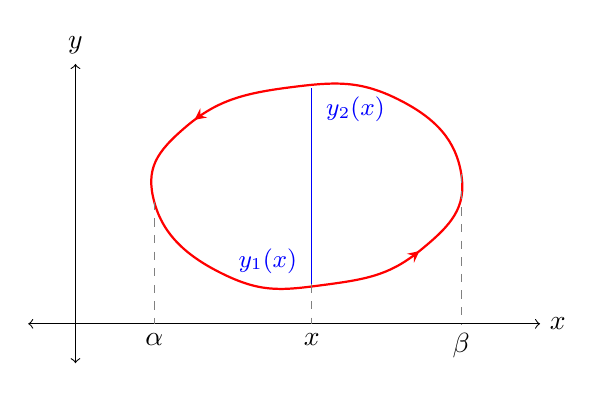
\begin{tikzpicture}[scale=1.0,
			decoration = {markings, mark=at position 0.25 with {\arrow{stealth}},
			              mark=at position 0.75 with {\arrow{stealth}}}]

			% draw axes
			\draw [<->] (-0.6, 0) -- (5.9, 0) node [right] {$x$};
			\draw [<->] (0, -0.5) -- (0, 3.3) node [above] {$y$};

			% draw the convex curve
			\draw [thick, red, postaction={decorate}] plot [smooth cycle, tension=0.8] coordinates {(1.0,1.55) (1.9,0.62) (3.2,0.5) (4.4,0.95) (4.9,1.9) (4.1,2.85) (2.7,3.0) (1.4,2.5)};

			\draw [dashed, gray] (4.9, 1.9) -- (4.9, 0) node [black, below] {$\beta$};
			\draw [dashed, gray] (1.0, 1.55) -- (1.0, 0) node [black, below] {$\alpha$};

			% a vertical slice
			\draw [thin, blue] (3.0, 0.5) -- (3.0, 3.0);
			\node [blue, right, font=\small] at (3.06, 2.72) {$y_2(x)$};
			\node [blue, left, font=\small] at (2.94, 0.80) {$y_1(x)$};
			\node [below] at (3.0, 0) {$x$};
			\draw [dashed, gray] (3.0, 0.5) -- (3.0, 0);
		\end{tikzpicture}
	\end{center}
	On the $x$-axis, we have minimal and maximal values $\alpha$ and $\beta$, and a simple closed curve $C$ with the given orientation. The $x$ coordinate monotonically increases from $\alpha \to \beta$ along the lower arc, and then decreases from $\beta \to \alpha$ along the upper arc.

	Given $x \in (\alpha, \beta)$, there are two points of the curve above $x$, at heights $y_1(x) < y_2(x)$, and from this we can write down the area as
	$$
	A[y] = \int_{\alpha}^{\beta} (y_2(x) - y_1(x)) \dd x = -\oint_C y \dd x,
	$$
	the sign being fixed by the orientation, and our perimeter constraint as
	$$
	L[y] = \oint_C \dd \ell = \oint_C \sqrt{1 + (y')^2} \dd x = L
	$$
	being constant.

	We now want to extremize $A - \lambda L$, and so we define
	$$
	h = y - \lambda \sqrt{1 + (y')^2},
	$$
	so that we can then try to solve the Euler-Lagrange equations (not worrying about the boundary term in the derivation of the Euler-Lagrange equations, as $C$ has no boundary).

	Since this has no dependence on $x$, we can use one of our first integrals. We know that $\partial h/\partial x = 0$, and also that
	\begin{align*}
		k &= h - y' \frac{\partial h}{\partial y'} \\
		  &= y - \lambda \sqrt{1 + (y')^2} + y' \lambda \frac{y'}{\sqrt{1 + (y')^2}}\\
		  &= y - \frac{\lambda}{\sqrt{1 + (y')^2}},
	\end{align*}
	for a constant $k$. Thus
	$$
	(y')^2 = \frac{\lambda^2}{(y - k)^2} - 1,
	$$
	which is separable. Writing $u = y - k$ we get $\dd x = \pm u\dd u/\sqrt{\lambda^2 - u^2}$, and integrating gives $x - x_0 = \mp\sqrt{\lambda^2 - u^2}$. Squaring and rearranging, the solution is
	$$
	(x - x_0)^2 + (y - y_0)^2 = \lambda^2,
	$$
	which is a circle of radius $\lambda$. Then $2\pi \lambda = L$ gives $\lambda = L/2\pi$. This is a necessary (but not sufficient) condition for our solution, so the circle is the only candidate.

	Notice that the Lagrange multiplier is here exactly the radius of the optimal circle, and hence that $\dd A/\dd L = \lambda$ -- which is easily checked directly, since $A = L^2/4\pi$. This is our general interpretation of the multiplier as a rate of change of the optimal value with the constraint, in action.
\end{example}

\subsection{Pointwise Constraints}

The constraint in an isoperimetric problem is a single number. Sometimes instead we want a constraint to hold at \emph{every} point of the curve -- for instance, that the curve lie on a given surface. In that case a single multiplier is not enough; we need a multiplier \emph{function} $\lambda(t)$, one for each point.

\begin{example}[Geodesics on a General Surface]
	Let $\Sigma = \{\vv{x} \in \R^3 : g(\vv{x}) = 0\}$ be a surface, and let $A, B \in \Sigma$. To find the geodesics between them, parameterize a path by $t \in [0,1]$ with $\vv{x}(0) = A$, $\vv{x}(1) = B$, and extremize
	$$
	\Phi[\vv{x}, \lambda] = \int_0^1\left\{\sqrt{\dot x_1^2 + \dot x_2^2 + \dot x_3^2} - \lambda(t)g(\vv{x})\right\}\dd t.
	$$
	Treating $\lambda$ as a fourth dependent variable, the Euler--Lagrange equation for $\lambda$ is
	$$
	\frac{\dd}{\dd t}\frac{\partial h}{\partial \dot\lambda} - \frac{\partial h}{\partial \lambda} = 0,
	$$
	and since $h$ does not involve $\dot \lambda$ at all, this just says $g(\vv x) = 0$ for all $t$ -- the constraint, as required. Varying the $x_i$ gives
	$$
	\frac{\dd}{\dd t}\left(\frac{\dot x_i}{\sqrt{\dot x_1^2 + \dot x_2^2 + \dot x_3^2}}\right) + \lambda \frac{\partial g}{\partial x_i} = 0.
	$$
	If we parameterize by arclength the square root is $1$, and the equation says $\ddot{\vv{x}} = -\lambda \nabla g$: the acceleration of a geodesic is always \emph{normal} to the surface. In other words, a geodesic is a curve which does not turn within the surface -- it only bends as much as the surface forces it to. This is a very clean characterisation, and one which the reader will meet again in Differential Geometry.

	Of course, we could instead have solved the constraint $g = 0$ by parameterizing $\Sigma$ explicitly, as we did for the sphere. Which approach is easier depends entirely on the surface.
\end{example}

\section{Soap Films and Hanging Chains}

We now pause the general theory to work through two classical problems in detail. Both are genuinely physical, both are solved by the hyperbolic cosine, and both have subtleties that the Euler--Lagrange equation alone does not reveal.

\subsection{Minimal Surfaces of Revolution}\label{sec:soap}

Dip two coaxial circular wire rings into soapy water and pull them apart. The soap film that forms is a surface of revolution, and since surface tension makes the film minimise its area, it is a solution of a variational problem.

\begin{center}
	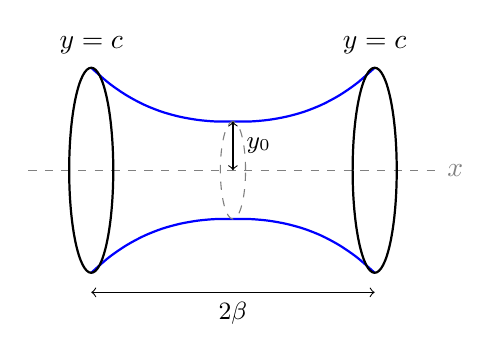
\begin{tikzpicture}[scale=1.0]
		% axis of revolution
		\draw [dashed, gray] (-2.6, 0) -- (2.6, 0) node [right] {$x$};

		% the catenoid profile y = 0.62 cosh(x/0.62), for x in [-1.8, 1.8]
		% precomputed points below
		\draw [thick, blue] plot [smooth] coordinates {(-1.800,1.302) (-1.575,1.106) (-1.350,0.951) (-1.125,0.831) (-0.900,0.742) (-0.675,0.680) (-0.450,0.640) (-0.225,0.620) (0.000,0.620) (0.225,0.620) (0.450,0.640) (0.675,0.680) (0.900,0.742) (1.125,0.831) (1.350,0.951) (1.575,1.106) (1.800,1.302)};
		\draw [thick, blue] plot [smooth] coordinates {(-1.800,-1.302) (-1.575,-1.106) (-1.350,-0.951) (-1.125,-0.831) (-0.900,-0.742) (-0.675,-0.680) (-0.450,-0.640) (-0.225,-0.620) (0.000,-0.620) (0.225,-0.620) (0.450,-0.640) (0.675,-0.680) (0.900,-0.742) (1.125,-0.831) (1.350,-0.951) (1.575,-1.106) (1.800,-1.302)};

		% the two rings
		\draw [thick] (-1.8, 0) ellipse (0.28 and 1.302);
		\draw [thick] (1.8, 0) ellipse (0.28 and 1.302);
		% the waist
		\draw [dashed, gray] (0, 0) ellipse (0.16 and 0.620);

		\draw [<->] (0, 0) -- (0, 0.620);
		\node [right, font=\small] at (0.05, 0.32) {$y_0$};
		\node [above] at (-1.8, 1.35) {$y = c$};
		\node [above] at (1.8, 1.35) {$y = c$};
		\draw [<->] (-1.8, -1.55) -- (1.8, -1.55);
		\node [below, font=\small] at (0, -1.55) {$2\beta$};
	\end{tikzpicture}
\end{center}

Take the axis of revolution to be the $x$-axis, and let the film be the surface obtained by rotating a curve $y = y(x) > 0$ about it, with the rings at $x = \pm\beta$ both of radius $c$. The area of the surface of revolution is
$$
A[y] = \int_{-\beta}^{\beta} 2\pi y \sqrt{1 + (y')^2}\dd x,
$$
subject to $y(\pm\beta) = c$. Discarding the $2\pi$, the integrand $f = y\sqrt{1 + (y')^2}$ has no explicit $x$-dependence, so the Beltrami identity applies:
$$
y\sqrt{1 + (y')^2} - y'\frac{yy'}{\sqrt{1 + (y')^2}} = \frac{y}{\sqrt{1 + (y')^2}} = y_0
$$
for some constant $y_0 > 0$. Rearranging,
$$
y' = \pm\frac{\sqrt{y^2 - y_0^2}}{y_0},
$$
which separates. Substituting $y = y_0\cosh u$ gives $\dd x = y_0 \dd u$, so $u = (x - x_1)/y_0$ and
$$
y = y_0\cosh\left(\frac{x - x_1}{y_0}\right).
$$
This curve is a \vocab{catenary}, and the surface it sweeps out is a \vocab{catenoid}. By the symmetry of our boundary conditions, $x_1 = 0$, and $y_0$ is the radius of the narrowest part of the film -- its `waist'.

All that remains is to determine $y_0$, from
$$
c = y_0 \cosh\left(\frac{\beta}{y_0}\right).
$$
This is where it gets interesting. Let us scale so that $\beta = 1$, and ask how many solutions $y_0$ this equation has for given $c$. Consider the function $\Psi(y_0) = y_0\cosh(1/y_0)$: as $y_0 \to 0^+$ it blows up (since $\cosh$ beats the linear factor), and as $y_0 \to \infty$ it also blows up (since $\cosh \to 1$ and the linear factor wins). So $\Psi$ has a minimum somewhere in between.

\begin{center}
	\begin{tikzpicture}[scale=1.0]
		\draw [<->] (-0.3, 0) -- (4.4, 0) node [right] {$y_0$};
		\draw [<->] (0, -0.3) -- (0, 3.3) node [above] {$c$};

		% Psi(y0) = y0 cosh(1/y0), scaled: x = 2*y0, y = 1.35*Psi
		% precomputed
		\draw [thick, blue] plot [smooth] coordinates {(0.560,2.985) (0.600,2.750) (0.700,2.418) (0.800,2.221) (0.900,2.106) (1.000,2.043) (1.100,2.014) (1.200,2.010) (1.300,2.022) (1.400,2.048) (1.500,2.083) (1.700,2.174) (1.900,2.283) (2.100,2.404) (2.300,2.535) (2.500,2.672) (2.700,2.815) (2.900,2.963)};

		% minimum marker at y0 = 0.833 (x=1.666), Psi = 1.5089 (y=2.037)
		\node at (1.666, 2.037) [circle, fill, inner sep=1.3pt] {};
		\draw [dashed, gray] (1.666, 0) node [below, font=\small] {$\mu$} -- (1.666, 2.037);
		\draw [dashed, gray] (0, 2.037) node [left, font=\small] {$c_*$} -- (1.666, 2.037);

		% a level c > c* with two intersections
		\draw [dashed, red] (0, 2.55) -- (3.15, 2.55);
		\node [red, right, font=\small] at (3.2, 2.55) {$c > c_*$};
	\end{tikzpicture}
\end{center}

Differentiating,
$$
\Psi'(y_0) = \cosh\frac{1}{y_0} - \frac{1}{y_0}\sinh\frac{1}{y_0},
$$
which vanishes when $\coth(1/y_0) = 1/y_0$. Numerically this gives $y_0 = \mu \approx 0.833$, and $c_* = \Psi(\mu) \approx 1.509$. Hence:
\begin{itemize}
	\item If $c > c_*$, there are \emph{two} catenoids meeting the boundary conditions: a fat one with $y_0 > \mu$, and a thin one with $y_0 < \mu$.
	\item If $c = c_*$, there is exactly one.
	\item If $c < c_*$ -- that is, if the rings are pulled too far apart relative to their size -- there is \emph{no} solution at all.
\end{itemize}

This is our promised failure of existence and uniqueness for the boundary value problem, and it is physically real: pull the rings far enough apart and the soap film snaps.

\subsection{The Goldschmidt Solution}

But what happens then? Physically, the film collapses into two flat discs, one spanning each ring. This is called the \vocab{Goldschmidt solution}, and it is a perfectly good competitor of area $2\pi c^2$ -- but it is not a smooth surface of revolution, so the Euler--Lagrange equation never saw it.

\begin{center}
	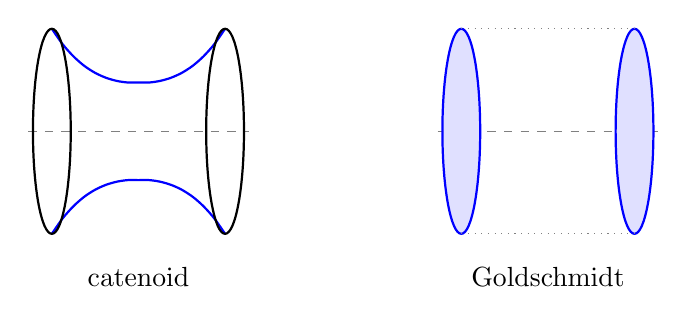
\begin{tikzpicture}[scale=1.0]
		\begin{scope}[shift={(-2.6,0)}]
			\draw [dashed, gray] (-1.4, 0) -- (1.4, 0);
			\draw [thick, blue] plot [smooth] coordinates {(-1.100,1.302) (-0.963,1.106) (-0.825,0.951) (-0.688,0.831) (-0.550,0.742) (-0.413,0.680) (-0.275,0.640) (-0.138,0.620) (0.000,0.620) (0.138,0.620) (0.275,0.640) (0.413,0.680) (0.550,0.742) (0.688,0.831) (0.825,0.951) (0.963,1.106) (1.100,1.302)};
			\draw [thick, blue] plot [smooth] coordinates {(-1.100,-1.302) (-0.963,-1.106) (-0.825,-0.951) (-0.688,-0.831) (-0.550,-0.742) (-0.413,-0.680) (-0.275,-0.640) (-0.138,-0.620) (0.000,-0.620) (0.138,-0.620) (0.275,-0.640) (0.413,-0.680) (0.550,-0.742) (0.688,-0.831) (0.825,-0.951) (0.963,-1.106) (1.100,-1.302)};
			\draw [thick] (-1.1, 0) ellipse (0.24 and 1.302);
			\draw [thick] (1.1, 0) ellipse (0.24 and 1.302);
			\node at (0, -1.85) {catenoid};
		\end{scope}
		\begin{scope}[shift={(2.6,0)}]
			\draw [dashed, gray] (-1.4, 0) -- (1.4, 0);
			\draw [thick, blue, fill=blue!12] (-1.1, 0) ellipse (0.24 and 1.302);
			\draw [thick, blue, fill=blue!12] (1.1, 0) ellipse (0.24 and 1.302);
			\draw [dotted, gray] (-1.1, 1.302) -- (1.1, 1.302);
			\draw [dotted, gray] (-1.1, -1.302) -- (1.1, -1.302);
			\node at (0, -1.85) {Goldschmidt};
		\end{scope}
	\end{tikzpicture}
\end{center}

Comparing the areas is a slightly delicate calculation, but the upshot is that as the rings are separated, the fat catenoid's area increases until, at a separation \emph{strictly less} than the critical one, it exceeds $2\pi c^2$. Past that point the Goldschmidt solution is the true global minimum even though a catenoid still exists.

There are two morals here, both worth remembering.
\begin{enumerate}[label=(\roman*)]
	\item The Euler--Lagrange equation only finds \emph{smooth} stationary points. Minima can occur at the boundary of the space of admissible functions -- just as, for functions on $\R^n$, minima can occur at the boundary of the domain.
	\item Of the two catenoids, the thin one ($y_0 < \mu$) turns out to be a saddle rather than a minimum: it is unstable, and a real soap film will never adopt it. We are not yet in a position to prove this, but we will develop the necessary tools in \autoref{sec:secondvar}.
\end{enumerate}

\subsection{The Hanging Chain}

A closely related problem: what shape does a heavy flexible chain of fixed length $L$ take when suspended from two points? The chain will hang so as to minimise its gravitational potential energy, subject to its length being fixed -- so this is an isoperimetric problem, and we need a Lagrange multiplier.

If the chain has uniform mass per unit length $\rho$ and hangs as $y = y(x)$ for $x \in [-\beta, \beta]$, its potential energy is
$$
V[y] = \int_{-\beta}^{\beta}\rho g\, y \sqrt{1 + (y')^2}\dd x,
$$
and the length constraint is
$$
L[y] = \int_{-\beta}^{\beta}\sqrt{1 + (y')^2}\dd x = L.
$$
So we extremize with the integrand
$$
h = (\rho g y - \lambda)\sqrt{1 + (y')^2}.
$$
But this is exactly the soap film integrand with $y$ replaced by $y - \lambda/\rho g$! So the calculation is identical, and the answer is a catenary,
$$
y = \frac{\lambda}{\rho g} + a \cosh\left(\frac{x - x_1}{a}\right),
$$
with $a$ and $\lambda$ fixed by the endpoint conditions and the length constraint. Here the multiplier $\lambda$ has a direct physical meaning: it is (up to sign) the horizontal tension in the chain.

That the soap film and the hanging chain give the same curve is not a coincidence -- both minimise $\int y \dd\ell$ -- but it is a pleasing one, and it is the reason the curve is called a catenary (from \emph{catena}, a chain).

It is a common misconception that a hanging chain is a parabola. It is not, though the two are close near the bottom: expanding,
$$
a\cosh\frac{x}{a} = a + \frac{x^2}{2a} + \frac{x^4}{24a^3} + \cdots,
$$
so they agree to second order and diverge thereafter. Galileo believed the curve was a parabola; the correct answer was found by Huygens, Leibniz and Johann Bernoulli in 1691.

\begin{center}
	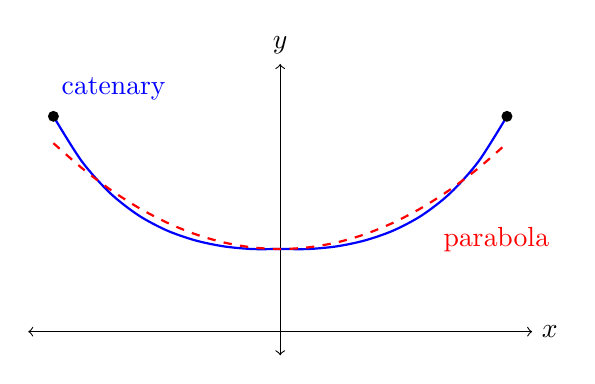
\begin{tikzpicture}[scale=1.0]
		\draw [<->] (-3.2, 0) -- (3.2, 0) node [right] {$x$};
		\draw [<->] (0, -0.3) -- (0, 3.4) node [above] {$y$};

		% catenary y = cosh(x) for x in [-1.6, 1.6], scaled: X = 1.8 x, Y = 1.05 cosh(x)
		\draw [thick, blue] plot [smooth] coordinates {(-2.880,2.735) (-2.520,2.164) (-2.160,1.760) (-1.800,1.478) (-1.440,1.286) (-1.080,1.160) (-0.720,1.084) (-0.360,1.050) (0.000,1.050) (0.360,1.050) (0.720,1.084) (1.080,1.160) (1.440,1.286) (1.800,1.478) (2.160,1.760) (2.520,2.164) (2.880,2.735)};
		% parabola through same endpoints: Y = 1.05 (1 + x^2/2), X = 1.8x  => Y = 1.05 + 0.525*(X/1.8)^2
		\draw [thick, red, dashed] plot [smooth] coordinates {(-2.880,2.394) (-2.520,2.079) (-2.160,1.806) (-1.800,1.575) (-1.440,1.386) (-1.080,1.239) (-0.720,1.134) (-0.360,1.071) (0.000,1.050) (0.360,1.071) (0.720,1.134) (1.080,1.239) (1.440,1.386) (1.800,1.575) (2.160,1.806) (2.520,2.079) (2.880,2.394)};

		\node [blue, right] at (-2.9, 3.08) {catenary};
		\node [red, below right] at (1.95, 1.45) {parabola};

		\node at (-2.880, 2.735) [circle, fill, inner sep=1.4pt] {};
		\node at (2.880, 2.735) [circle, fill, inner sep=1.4pt] {};
	\end{tikzpicture}
\end{center}

\subsection{Plateau's Problem and the Minimal Surface Equation}

Our soap film was a surface of revolution, which reduced the problem to one dependent variable. What if we dip an arbitrary closed wire loop into soapy water? The film that forms spans the loop and minimises area, and finding it is called \vocab{Plateau's problem}. This is a genuine multi-variable calculus of variations problem, and it is a good test of the machinery from the previous section.

Suppose the surface can be written as a graph $z = \phi(x, y)$ over a domain $\mathcal{D}$ in the plane, with $\phi$ prescribed on $\partial \mathcal D$ by the wire. Since $\dd z = \phi_x \dd x + \phi_y \dd y$, the line element on the surface is
$$
\dd s^2 = \left(1 + \phi_x^2\right)\dd x^2 + 2\phi_x\phi_y \dd x \dd y + \left(1 + \phi_y^2\right)\dd y^2 = g_{ij}\dd x^i \dd x^j,
$$
where
$$
g = \begin{pmatrix} 1 + \phi_x^2 & \phi_x\phi_y \\ \phi_x\phi_y & 1 + \phi_y^2\end{pmatrix}
$$
is the \vocab{first fundamental form} of the surface. The area element is $\dd A = \sqrt{\det g}\,\dd x\dd y$, and $\det g = 1 + \phi_x^2 + \phi_y^2$ (the cross terms cancel), so we wish to extremize
$$
A[\phi] = \iint_{\mathcal D}\sqrt{1 + \phi_x^2 + \phi_y^2}\dd x \dd y.
$$
Writing $h$ for the integrand, we have $\partial h/\partial \phi = 0$ and
$$
\frac{\partial h}{\partial \phi_x} = \frac{\phi_x}{\sqrt{1 + \phi_x^2 + \phi_y^2}}, \qquad \frac{\partial h}{\partial \phi_y} = \frac{\phi_y}{\sqrt{1 + \phi_x^2 + \phi_y^2}},
$$
so the Euler--Lagrange equation is
$$
\partial_x\left(\frac{\phi_x}{\sqrt{1 + \phi_x^2 + \phi_y^2}}\right) + \partial_y\left(\frac{\phi_y}{\sqrt{1 + \phi_x^2 + \phi_y^2}}\right) = 0.
$$
Expanding the derivatives and clearing the denominator gives the \vocab{minimal surface equation}
$$
\left(1 + \phi_y^2\right)\phi_{xx} - 2\phi_x\phi_y\phi_{xy} + \left(1 + \phi_x^2\right)\phi_{yy} = 0.
$$
This is a nonlinear second-order PDE, and it is not one we can solve in general. Two observations, though.

First, if the surface is nearly flat, so that $|\nabla\phi| \ll 1$, we may drop the quadratic terms and are left with
$$
\phi_{xx} + \phi_{yy} = 0,
$$
Laplace's equation again. This is the same linearisation that turns the exact equations of a stretched membrane into the wave equation studied in the Methods course.

Second, we can solve it exactly in the circularly symmetric case, and recover the catenoid. Put $z = \phi(r)$ with $r = \sqrt{x^2 + y^2}$. Then $\phi_x = z' x/r$ and $\phi_y = z' y/r$, and computing the second derivatives and substituting reduces the minimal surface equation to
$$
r z'' + z' + (z')^3 = 0.
$$
Setting $w = z'$ and multiplying through by $w$, this becomes
$$
\frac{1}{2}r\frac{\dd (w^2)}{\dd r} + w^2 + w^4 = 0,
$$
and with $u = w^2$ this is separable:
$$
\frac{\dd u}{u(1 + u)} = -\frac{2\dd r}{r}.
$$
Integrating with partial fractions gives $u/(1+u) = r_0^2/r^2$ for a constant $r_0$, so $w^2 = r_0^2/(r^2 - r_0^2)$ and
$$
\frac{\dd z}{\dd r} = \frac{r_0}{\sqrt{r^2 - r_0^2}} \implies z - z_0 = r_0 \operatorname{arcosh}\left(\frac{r}{r_0}\right).
$$
Inverting,
$$
r = r_0\cosh\left(\frac{z - z_0}{r_0}\right),
$$
which is exactly the catenoid we found in \autoref{sec:soap} -- reassuringly, since the two calculations describe the same soap film. It is always worth doing a problem twice when the two routes are this different.

\section{Hamilton's Principle and Lagrangian Mechanics}\label{sec:hamilton}

We now turn to the most celebrated application of everything we have built: the reformulation of classical mechanics as a variational principle. The payoff is enormous. Newton's laws are tied to Cartesian coordinates and inertial frames, and become painful the moment we have constraints (a bead on a wire, a pendulum on a pendulum). The variational formulation is coordinate-free, handles constraints gracefully, and -- through Noether's theorem -- hands us the conservation laws for free.

\subsection{The Principle of Least Action}

\begin{definition}[Lagrangian and Action]
	For a particle of mass $m$ moving in $\R^3$ under a potential $V(\vv x)$, with kinetic energy $T = \frac12 m|\dot{\vv x}|^2$, the \vocab{Lagrangian} is
	$$
	L(\vv x, \dot{\vv x}, t) = T - V,
	$$
	and the \vocab{action} of a path $\vv x(t)$ between times $t_1$ and $t_2$ is
	$$
	S[\vv x] = \int_{t_1}^{t_2}L(\vv x, \dot{\vv x}, t)\dd t.
	$$
\end{definition}

\begin{law}[Hamilton's Principle]
	The path actually taken by the particle between two fixed configurations at times $t_1$ and $t_2$ is a stationary point of the action.
\end{law}

The difference $T - V$ looks strange -- one would more naturally write down $T + V$, the energy. But it is $T - V$ that works, and we can check this immediately.

\begin{center}
	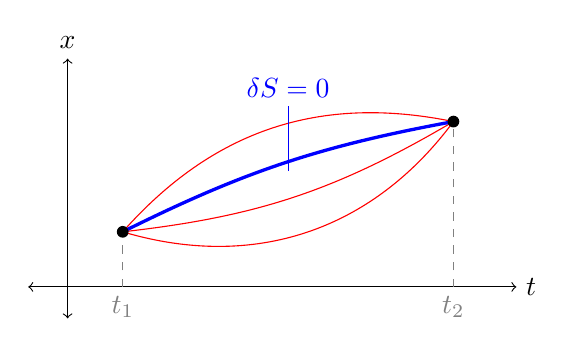
\begin{tikzpicture}[scale=1.0]
		\draw [<->] (-0.5, 0) -- (5.7, 0) node [right] {$t$};
		\draw [<->] (0, -0.4) -- (0, 2.9) node [above] {$x$};

		\coordinate (p) at (0.7, 0.7);
		\coordinate (q) at (4.9, 2.1);

		\draw [dashed, gray] (0.7, 0) node [below] {$t_1$} -- (p);
		\draw [dashed, gray] (4.9, 0) node [below] {$t_2$} -- (q);

		% competing paths
		\draw [thin, red] (p) to [bend left=30] (q);
		\draw [thin, red] (p) to [bend right=35] (q);
		\draw [thin, red] (p) to [bend right=12] (q);
		% the true path
		\draw [very thick, blue] (p) to [bend left=8] (q);
		\draw [thin, blue] (2.8, 1.47) -- (2.8, 2.30);
		\node [blue, above] at (2.8, 2.28) {$\delta S = 0$};

		\node at (p) [circle, fill, inner sep=1.5pt] {};
		\node at (q) [circle, fill, inner sep=1.5pt] {};
	\end{tikzpicture}
\end{center}

\begin{theorem}
	Hamilton's principle is equivalent to Newton's second law $m\ddot{\vv x} = -\nabla V$.
\end{theorem}
\begin{proof}
	This is the Euler--Lagrange equations for several dependent variables from \autoref{sec:multidep}, with $x$ replaced by $t$ and $y_i$ by $x_i$. We have
	$$
	L = \frac{1}{2}m\left(\dot x_1^2 + \dot x_2^2 + \dot x_3^2\right) - V(\vv x),
	$$
	so $\partial L/\partial \dot x_i = m \dot x_i$ and $\partial L/\partial x_i = -\partial V/\partial x_i$. The Euler--Lagrange equations
	$$
	\frac{\dd}{\dd t}\left(\frac{\partial L}{\partial \dot x_i}\right) - \frac{\partial L}{\partial x_i} = 0
	$$
	therefore read $m\ddot x_i = -\partial V/\partial x_i$, which is Newton's second law.
\end{proof}

So the mysterious minus sign is exactly what is needed to produce `mass times acceleration equals force'. Two immediate remarks. First, `least action' is a misnomer -- the action is stationary, and is often a saddle rather than a minimum. Second, the Euler--Lagrange equations retain their form under \emph{any} change of coordinates, since our derivation never used what the coordinates meant. This is what makes the formulation so powerful.

\subsection{Generalised Coordinates}

Suppose we have $N$ particles in $\R^3$. Rather than tracking $N$ vectors, we regard the state of the whole system as a single point in $\R^{3N}$, called the \vocab{configuration space}. If the system is subject to constraints -- rigid rods, beads on wires, and so on -- the accessible configurations form a lower-dimensional surface inside $\R^{3N}$, and we may choose any convenient coordinates $q_1, \dots, q_n$ on it. These are the \vocab{generalised coordinates}, and $n$ is the number of degrees of freedom.

The great advantage is that the constraint forces disappear entirely: we simply write the kinetic and potential energies in terms of the $q_i$, form
$$
L = L(q_i, \dot q_i, t),
$$
and write down the Euler--Lagrange equations
$$
\frac{\dd}{\dd t}\left(\frac{\partial L}{\partial \dot q_i}\right) - \frac{\partial L}{\partial q_i} = 0.
$$
The quantity $p_i = \partial L/\partial \dot q_i$ is called the \vocab{generalised} (or \vocab{conjugate}) \vocab{momentum} associated with $q_i$; for a Cartesian coordinate it is the ordinary momentum $m\dot x$.

\begin{example}[The Simple Pendulum]
	A mass $m$ swings on a light rod of length $\ell$. There is one degree of freedom, the angle $\theta$ from the downward vertical. The speed of the mass is $\ell\dot\theta$ and its height above the lowest point is $\ell(1 - \cos\theta)$, so
	$$
	L = \frac{1}{2}m\ell^2\dot\theta^2 - mg\ell(1 - \cos\theta).
	$$
	Then $\partial L/\partial \dot\theta = m\ell^2\dot\theta$ and $\partial L/\partial\theta = -mg\ell\sin\theta$, so the equation of motion is
	$$
	m\ell^2\ddot\theta = -mg\ell\sin\theta \implies \ddot\theta = -\frac{g}{\ell}\sin\theta,
	$$
	in two lines and with no mention of the tension in the rod. Doing this with Newton's laws requires resolving forces along and perpendicular to the rod, and is distinctly more work.
\end{example}

\begin{example}[Motion in a Central Force]
	Consider a particle moving in a plane under a central potential $V(r)$. Using plane polar coordinates $(r, \theta)$, the velocity has components $\dot r$ and $r\dot\theta$, so
	$$
	L = \frac{1}{2}m\left(\dot r^2 + r^2\dot\theta^2\right) - V(r).
	$$
	Now $\theta$ is cyclic -- it does not appear in $L$, only $\dot\theta$ does -- so we immediately get a first integral,
	$$
	\frac{\partial L}{\partial \dot\theta} = m r^2\dot\theta = \text{constant},
	$$
	which is conservation of angular momentum. Also $L$ has no explicit $t$-dependence, so the Beltrami identity applies (in its several-variable form):
	\begin{align*}
		\text{constant} &= \dot r \frac{\partial L}{\partial \dot r} + \dot\theta\frac{\partial L}{\partial \dot\theta} - L \\
		&= m\dot r^2 + mr^2\dot\theta^2 - \frac12 m \dot r^2 - \frac12 mr^2\dot\theta^2 + V(r) \\
		&= \frac{1}{2}m\left(\dot r^2 + r^2\dot\theta^2\right) + V(r),
	\end{align*}
	which is $T + V$: conservation of energy. So both conservation laws for the Kepler problem drop out of the structure of $L$ without solving anything.
\end{example}

\begin{example}[The Double Pendulum]
	To see how little the method cares about complexity, consider a pendulum of length $\ell_1$ carrying a mass $m_1$, from which hangs a second pendulum of length $\ell_2$ carrying $m_2$. Let $\theta_1, \theta_2$ be the angles of the two rods from the vertical; these are our generalised coordinates, and there are two degrees of freedom.

	The position of the first mass is $\ell_1(\sin\theta_1, -\cos\theta_1)$ and of the second is that plus $\ell_2(\sin\theta_2, -\cos\theta_2)$. Differentiating and squaring,
	$$
	T = \frac{1}{2}(m_1 + m_2)\ell_1^2\dot\theta_1^2 + \frac{1}{2}m_2\ell_2^2\dot\theta_2^2 + m_2\ell_1\ell_2 \dot\theta_1\dot\theta_2\cos(\theta_1 - \theta_2),
	$$
	while the potential energy is
	$$
	V = -(m_1 + m_2)g\ell_1\cos\theta_1 - m_2 g \ell_2\cos\theta_2.
	$$
	Writing $L = T - V$ and grinding out $\frac{\dd}{\dd t}(\partial L/\partial \dot\theta_i) = \partial L/\partial\theta_i$ gives the (famously chaotic) equations of motion. The point is not the equations, which are unpleasant, but that we obtained them by writing down two energies and differentiating. There is no need to think about the forces in the rods at all, which is what makes a Newtonian treatment of this system so disagreeable.

	Note also that $L$ has no explicit $t$-dependence, so energy is conserved; but no coordinate is cyclic, so there is no second conserved quantity. Two degrees of freedom and only one conservation law is, roughly speaking, why the system is chaotic.
\end{example}

That last example is suggestive. A missing coordinate gave conservation of angular momentum; a missing time gave conservation of energy. There is a general principle lurking here, and it is due to Emmy Noether.

\subsection{Noether's Theorem}\label{sec:noether}

The key idea is to replace `the Lagrangian does not depend on $\theta$' -- which is a statement about a particular coordinate system -- with the coordinate-free statement `the Lagrangian is invariant under rotations'. Symmetries, rather than missing variables.

\begin{definition}[Continuous Symmetry]
	Consider a functional $F[\vv y] = \int_\alpha^\beta f(y_i, y_i', x)\dd x$. A \vocab{one-parameter family of transformations} is a smooth map
	$$
	y_i(x) \longmapsto Y_i(x, s), \qquad Y_i(x, 0) = y_i(x),
	$$
	for $s$ in some interval around $0$. It is a \vocab{continuous symmetry} of $f$ if
	$$
	\frac{\partial}{\partial s}f\left(Y_i(x, s), Y_i'(x, s), x\right) = 0
	$$
	for all $s$, where $' = \partial/\partial x$ as usual.
\end{definition}

\begin{theorem}[Noether's Theorem]
	Let $Y_i(x, s)$ be a continuous symmetry of $f$. Then, along any solution of the Euler--Lagrange equations,
	$$
	\left.\sum_{i=1}^n\frac{\partial f}{\partial y_i'}\frac{\partial Y_i}{\partial s}\right|_{s = 0}
	$$
	is constant, i.e.\ it is a first integral.
\end{theorem}
\begin{proof}
	The proof is three lines of chain rule, and is worth following carefully. Using the summation convention, and evaluating everything at $s = 0$,
	\begin{align*}
		0 &= \left.\frac{\partial f}{\partial s}\right|_{s = 0} \\
		&= \left.\frac{\partial f}{\partial y_i}\frac{\partial Y_i}{\partial s}\right|_{s=0} + \left.\frac{\partial f}{\partial y_i'}\frac{\partial Y_i'}{\partial s}\right|_{s=0} \\
		&= \left.\left[\frac{\dd}{\dd x}\left(\frac{\partial f}{\partial y_i'}\right)\frac{\partial Y_i}{\partial s} + \frac{\partial f}{\partial y_i'}\frac{\dd}{\dd x}\left(\frac{\partial Y_i}{\partial s}\right)\right]\right|_{s=0} \\
		&= \frac{\dd}{\dd x}\left.\left[\frac{\partial f}{\partial y_i'}\frac{\partial Y_i}{\partial s}\right]\right|_{s=0}.
	\end{align*}
	In the third line we used the Euler--Lagrange equation to replace $\partial f/\partial y_i$, and swapped the order of the mixed partial derivatives $\partial_s\partial_x = \partial_x\partial_s$; the last line is the product rule read backwards. Integrating, the bracket is constant.
\end{proof}

The statement is short but the content is remarkable: \emph{every continuous symmetry of a physical system yields a conserved quantity}. Let us see it work.

\begin{example}[Conservation of Momentum]
	Let $\vv y = (y, z)$ and
	$$
	f = \frac{1}{2}(y')^2 + \frac{1}{2}(z')^2 - V(y - z),
	$$
	which describes two particles interacting through a potential depending only on their separation. Consider translating both by the same amount:
	$$
	Y = y + s, \qquad Z = z + s.
	$$
	Then $Y' = y'$, $Z' = z'$, and $Y - Z = y - z$, so $f$ is unchanged and this is a symmetry. Since $\partial Y/\partial s = \partial Z/\partial s = 1$, Noether's theorem gives the first integral
	$$
	\frac{\partial f}{\partial y'}\cdot 1 + \frac{\partial f}{\partial z'}\cdot 1 = y' + z' = \text{constant},
	$$
	which is conservation of total momentum. The physical statement is that space is homogeneous -- it does not matter \emph{where} the experiment is performed.
\end{example}

\begin{example}[Conservation of Angular Momentum]
	Take the central force Lagrangian $L = \frac12 m(\dot r^2 + r^2\dot\theta^2) - V(r)$ and the rotation
	$$
	R = r, \qquad \Theta = \theta + s.
	$$
	This leaves $L$ unchanged since $L$ does not involve $\theta$, so it is a symmetry, and Noether's theorem gives
	$$
	\frac{\partial L}{\partial \dot r}\cdot 0 + \frac{\partial L}{\partial \dot\theta}\cdot 1 = mr^2\dot\theta = \text{constant},
	$$
	as we found before. The physical statement is that space is isotropic.
\end{example}

\begin{remark}
	Conservation of energy also comes from a symmetry -- invariance under time translation -- but this is a symmetry of the \emph{independent} variable rather than the dependent ones, and so is not literally covered by the version of Noether's theorem we proved. In our framework it appears instead as the Beltrami identity, which is the same statement in disguise. A more general version of Noether's theorem handles both at once.
\end{remark}

\subsection{The Hamiltonian}

We saw in \autoref{prop:beltrami} that when $L$ has no explicit time dependence, the quantity
$$
H = \sum_i \dot q_i \frac{\partial L}{\partial \dot q_i} - L = \sum_i p_i \dot q_i - L
$$
is conserved. But look at the right hand side: this is exactly the Legendre transform of $L$ with respect to $\dot{\vv q}$.

\begin{definition}[Hamiltonian]
	The \vocab{Hamiltonian} is the Legendre transform of the Lagrangian in the velocities,
	$$
	H(\vv q, \vv p, t) = \sup_{\vv v}\left(\vv p \cdot \vv v - L(\vv q, \vv v, t)\right) = \vv p \cdot \dot{\vv q} - L,
	$$
	where $\dot{\vv q}$ is expressed in terms of $\vv p$ by inverting $p_i = \partial L/\partial \dot q_i$.
\end{definition}

Convexity of $L$ in $\dot{\vv q}$ -- which for $T = \frac12 m|\dot{\vv q}|^2$ is automatic -- is exactly what guarantees this inversion is possible, and this is why we spent time on the Legendre transform earlier.

\begin{example}
	Take $L = \frac12 m|\dot{\vv q}|^2 - V(\vv q)$. Then $\vv p = \partial L/\partial \dot{\vv q} = m\dot{\vv q}$, so $\dot{\vv q} = \vv p/m$, and
	\begin{align*}
		H &= \vv p \cdot \frac{\vv p}{m} - \left(\frac{1}{2}m\frac{|\vv p|^2}{m^2} - V(\vv q)\right) \\
		&= \frac{|\vv p|^2}{2m} + V(\vv q) = T + V.
	\end{align*}
	So the Hamiltonian is the total energy -- but expressed in terms of momentum rather than velocity, which is the whole point.
\end{example}

The change of variables from $(\vv q, \dot{\vv q})$ to $(\vv q, \vv p)$ does more than tidy the energy; it transforms the equations of motion into a strikingly symmetric first-order system.

\begin{theorem}[Hamilton's Equations]
	If $L$ satisfies the Euler--Lagrange equations, then
	$$
	\dot q_i = \frac{\partial H}{\partial p_i}, \qquad \dot p_i = -\frac{\partial H}{\partial q_i}, \qquad \frac{\partial H}{\partial t} = -\frac{\partial L}{\partial t}.
	$$
\end{theorem}
\begin{proof}
	The slick proof is to compute the differential of $H = p_i\dot q_i - L$ in two ways. Regarding $H$ as a function of $(\vv q, \vv p, t)$,
	$$
	\dd H = \frac{\partial H}{\partial q_i}\dd q_i + \frac{\partial H}{\partial p_i}\dd p_i + \frac{\partial H}{\partial t}\dd t.
	$$
	On the other hand, differentiating $p_i \dot q_i - L(\vv q, \dot{\vv q}, t)$ directly,
	$$
	\dd H = p_i \dd\dot q_i + \dot q_i \dd p_i - \frac{\partial L}{\partial q_i}\dd q_i - \frac{\partial L}{\partial \dot q_i}\dd \dot q_i - \frac{\partial L}{\partial t}\dd t.
	$$
	The first and fourth terms cancel, since $p_i = \partial L/\partial \dot q_i$ -- this cancellation is the magic of the Legendre transform, and it is why $H$ genuinely is a function of $\vv p$ and not of $\dot{\vv q}$. For the third term, the Euler--Lagrange equation gives
	$$
	\frac{\partial L}{\partial q_i} = \frac{\dd}{\dd t}\frac{\partial L}{\partial \dot q_i} = \dot p_i.
	$$
	So
	$$
	\dd H = \dot q_i \dd p_i - \dot p_i \dd q_i - \frac{\partial L}{\partial t}\dd t,
	$$
	and comparing coefficients with the first expression gives the result.
\end{proof}

\begin{example}[The Harmonic Oscillator in Phase Space]
	Take $L = \frac12 m\dot q^2 - \frac12 m\omega^2 q^2$. Then $p = m\dot q$, and
	$$
	H = \frac{p^2}{2m} + \frac{1}{2}m\omega^2 q^2.
	$$
	Hamilton's equations are
	$$
	\dot q = \frac{\partial H}{\partial p} = \frac{p}{m}, \qquad \dot p = -\frac{\partial H}{\partial q} = -m\omega^2 q,
	$$
	which combine to give $\ddot q = -\omega^2 q$ as expected. But the first-order form has an advantage: since $H$ is conserved, every trajectory lies on a level set of $H$, that is, on an ellipse
	$$
	\frac{p^2}{2m} + \frac{1}{2}m\omega^2q^2 = E
	$$
	in the $(q, p)$ plane. We can therefore read off the qualitative behaviour of every solution -- they all go round and round -- without solving anything at all. This is the typical use of the Hamiltonian formulation: it turns dynamics into geometry in phase space.
\end{example}

We have traded $n$ second-order equations for $2n$ first-order ones, which carry the same amount of information (the same number of constants of integration). The space of pairs $(\vv q, \vv p)$ is called \vocab{phase space}, and solutions of Hamilton's equations are \emph{trajectories} in it. The symmetry between $q$ and $p$ in these equations -- broken only by a minus sign -- is the starting point of a very rich theory, and it is the form of mechanics which passes most directly into quantum mechanics.

\begin{remark}
	Hamilton's equations can also be obtained variationally, which is rather satisfying. Consider the functional on phase space
	$$
	S[\vv q, \vv p] = \int_{t_1}^{t_2}\left(p_i \dot q_i - H(\vv q, \vv p, t)\right)\dd t,
	$$
	and treat $\vv q$ and $\vv p$ as independent. Since the integrand contains no $\dot p_i$, the Euler--Lagrange equation for $p_i$ is simply $\partial f/\partial p_i = 0$, giving $\dot q_i = \partial H/\partial p_i$. The equation for $q_i$ gives $-\partial H/\partial q_i - \dd p_i/\dd t = 0$, which is the second of Hamilton's equations.
\end{remark}

\section{Eigenvalue Problems and the Rayleigh--Ritz Method}\label{sec:rayleigh}

We now return to constrained variational problems, and to an application which is of great practical importance: estimating eigenvalues. The key observation is that eigenvalues of certain differential operators are the minima of an associated functional -- and because minima are easy to bound from above (just guess something!), this gives a genuinely useful computational method.

\subsection{The Sturm--Liouville Problem}

\begin{example}[The Sturm--Liouville Problem]
	Let $\rho(x) > 0$ be some known function for $x \in [\alpha, \beta]$, and let $\sigma(x)$ be another function. We consider the functional
	$$
	F[y] = \int_{\alpha}^{\beta} \left[\rho \cdot (y')^2 + \sigma \cdot y^2\right] \dd x,
	$$
	and we want to minimize $F$ subject to the normalisation
	$$
	G[y] = \int_\alpha^{\beta} y^2 \dd x = 1,
	$$
	and the boundary conditions $y(\alpha) = y(\beta) = 0$.

	We define the functional
	$$
	\Phi[y; \lambda] = F[y] - \lambda \left(G[y] - 1\right),
	$$
	whose integrand is $h = \rho (y')^2 + \sigma y^2 - \lambda y^2$ (plus a constant, which does not affect the equations). Then
	$$
	\frac{\partial h}{\partial y'} = 2\rho y', \qquad \frac{\partial h}{\partial y} = 2\sigma y - 2\lambda y,
	$$
	and the Euler--Lagrange equation $\frac{\dd}{\dd x}(\partial h/\partial y') = \partial h /\partial y$ becomes, after dividing by $2$,
	$$
	-\frac{\dd}{\dd x}\left(\rho \frac{\dd y}{\dd x}\right) + \sigma y = \lambda y.
	$$
	Writing $\mathcal{L}$ for the operator on the left, this is
	$$
	\mathcal{L}y = \lambda y,
	$$
	an eigenvalue problem, and $\mathcal{L}$ is the \vocab{Sturm--Liouville operator} familiar from the Methods course\footnote{The reader who wants the full theory -- self-adjointness, orthogonality and completeness of the eigenfunctions, and the eigenfunction expansion -- is referred to the Sturm--Liouville chapter of my Methods notes. We will use those facts here without proof.}. So the Lagrange multiplier of our constrained problem is precisely the eigenvalue.

	If $\rho = 1$ this is the time-independent Schr\"odinger equation with potential $\sigma$, which we will return to shortly.
\end{example}

This connection is worth stating as a theorem, because it is the engine of everything that follows.

\begin{theorem}[Eigenvalues as Minima]\label{thm:rayleigh}
	Let $\mathcal{L}y = -(\rho y')' + \sigma y$ with $\rho > 0$, acting on functions with $y(\alpha) = y(\beta) = 0$, and let its eigenvalues be $\lambda_1 \leq \lambda_2 \leq \cdots$ with eigenfunctions $y_1, y_2, \dots$. Define the \vocab{Rayleigh quotient}
	$$
	\mathcal{R}[y] = \frac{F[y]}{G[y]} = \frac{\displaystyle\int_\alpha^\beta \left(\rho (y')^2 + \sigma y^2\right)\dd x}{\displaystyle\int_\alpha^\beta y^2 \dd x}.
	$$
	Then $\lambda_1 = \min \mathcal{R}[y]$, the minimum being over all admissible $y \not\equiv 0$, and it is attained at $y = y_1$.
\end{theorem}
\begin{proof}
	First, note that $\mathcal{R}$ is unaffected by scaling $y$, so we may as well impose $G[y] = 1$; then $\mathcal{R}[y] = F[y]$.

	Suppose $y$ is a stationary point of $F$ subject to $G = 1$, with multiplier $\lambda$. Multiplying the Euler--Lagrange equation $-(\rho y')' + \sigma y = \lambda y$ by $y$ and integrating,
	$$
	\int_\alpha^\beta\left(-y(\rho y')' + \sigma y^2\right)\dd x = \lambda \int_\alpha^\beta y^2\dd x = \lambda.
	$$
	Integrating the first term by parts,
	$$
	\int_\alpha^\beta \left(\rho (y')^2 + \sigma y^2\right)\dd x - \cancel{\left[y\rho y'\right]_\alpha^\beta} = \lambda,
	$$
	the boundary term vanishing since $y(\alpha) = y(\beta) = 0$. So $F[y] = \lambda$: \emph{the value of the functional at a stationary point is the corresponding eigenvalue}. Hence the smallest value of $\mathcal{R}$ over stationary points is the smallest eigenvalue.

	It remains to see that the minimum over \emph{all} $y$ is attained at a stationary point, which follows by expanding an arbitrary $y$ in the eigenfunctions. Writing $y = \sum_n c_n y_n$ with the $y_n$ orthonormal (which we may do by the completeness of the eigenfunctions, proved in the Methods course), the same integration by parts gives
	$$
	F[y] = \sum_n \lambda_n c_n^2, \qquad G[y] = \sum_n c_n^2,
	$$
	so that
	$$
	\mathcal{R}[y] = \frac{\sum_n \lambda_n c_n^2}{\sum_n c_n^2} \geq \lambda_1,
	$$
	since every $\lambda_n \geq \lambda_1$. Equality holds exactly when $c_n = 0$ for all $n$ with $\lambda_n > \lambda_1$, i.e.\ when $y$ is a ground state.
\end{proof}

The last display deserves emphasis. It says that $\mathcal{R}[y]$ is a \emph{weighted average} of the eigenvalues, with weights $c_n^2$ given by how much of each eigenfunction $y$ contains. An average of numbers is at least the smallest of them, and that is the entire content of the variational principle.

\subsection{The Rayleigh--Ritz Method}

Here is the practical consequence. Suppose we cannot solve $\mathcal{L}y = \lambda y$ exactly, but we would like to know $\lambda_1$. By \autoref{thm:rayleigh}, \emph{any} admissible function $y$ we care to write down gives an upper bound
$$
\lambda_1 \leq \mathcal{R}[y].
$$
So we take a \vocab{trial function} $y$ depending on a few free parameters, compute $\mathcal{R}[y]$, and minimise over the parameters. This is the \vocab{Rayleigh--Ritz method}. The more parameters we allow, the better the bound -- and the bound is always from above, so we always know which way we are wrong.

\begin{center}
	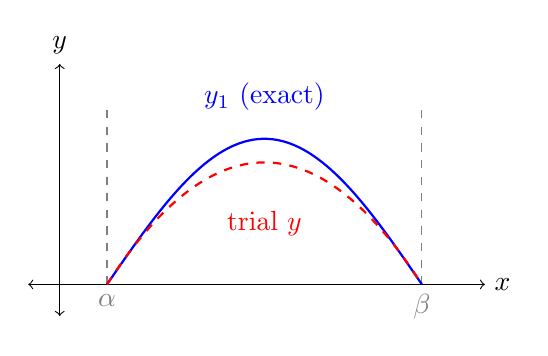
\begin{tikzpicture}[scale=1.0]
		\draw [<->] (-0.4, 0) -- (5.4, 0) node [right] {$x$};
		\draw [<->] (0, -0.4) -- (0, 2.8) node [above] {$y$};
		\draw [dashed, gray] (0.6, 0) node [below] {$\alpha$} -- (0.6, 2.3);
		\draw [dashed, gray] (4.6, 0) node [below] {$\beta$} -- (4.6, 2.3);

		% true eigenfunction: sin bump
		\draw [thick, blue, smooth, samples=60, domain=0.6:4.6] plot (\x, {1.85*sin(180*(\x-0.6)/4)});
		\node [blue, above] at (2.6, 2.08) {$y_1$ (exact)};

		% trial function: a parabola through the same endpoints, slightly different
		\draw [thick, red, dashed, smooth, samples=60, domain=0.6:4.6] plot (\x, {1.55*(\x-0.6)*(4.6-\x)/4});
		\node [red, below] at (2.6, 1.05) {trial $y$};
	\end{tikzpicture}
\end{center}

\begin{example}
	Let us estimate the lowest eigenvalue of $-y'' = \lambda y$ on $[0, 1]$ with $y(0) = y(1) = 0$. Of course we know the answer is $\lambda_1 = \pi^2 \approx 9.8696$, which makes this a good test.

	Take the simplest trial function vanishing at both ends, $y = x(1-x)$. Then $y' = 1 - 2x$, and
	$$
	\int_0^1 (y')^2\dd x = \int_0^1 (1-2x)^2\dd x = \frac{1}{3}, \qquad \int_0^1 y^2\dd x = \int_0^1 x^2(1-x)^2\dd x = \frac{1}{30}.
	$$
	So
	$$
	\lambda_1 \leq \frac{1/3}{1/30} = 10.
	$$
	This is within $1.5\%$ of the true value, from a one-line calculation with a function that is not even the right shape. The reason the method works so well is that $\mathcal{R}$ is \emph{stationary} at $y_1$, so an error of size $\epsilon$ in the trial function produces an error of only $O(\epsilon^2)$ in the estimate.

	If we want to do better we can add a parameter. Taking $y = x(1-x)(1 + ax)$ and minimising over $a$ gives $\lambda_1 \leq 9.8697$, correct to four decimal places.
\end{example}

\begin{remark}
	The method extends to higher eigenvalues. Since $\mathcal{R}[y] = \sum\lambda_n c_n^2/\sum c_n^2$, if we restrict to trial functions orthogonal to $y_1$ (so $c_1 = 0$) then the same argument gives $\lambda_2 = \min \mathcal{R}[y]$ over that restricted class, and so on. In practice one rarely knows $y_1$ exactly, which limits the usefulness -- but symmetry often helps. For instance, if the problem is symmetric about the midpoint then $y_1$ is even, so any odd trial function is automatically orthogonal to it and bounds $\lambda_2$.
\end{remark}

\subsection{Inequalities from Variational Principles}

The Rayleigh quotient can be read in the other direction. Instead of using known eigenvalues to bound $\mathcal{R}$, we can use a known eigenvalue to prove an inequality about \emph{all} functions -- and some rather famous inequalities arise this way.

\begin{theorem}[Poincar\'e--Wirtinger Inequality]
	Let $y \in C^1[0, L]$ with $y(0) = y(L) = 0$. Then
	$$
	\int_0^L (y')^2\dd x \geq \frac{\pi^2}{L^2}\int_0^L y^2 \dd x,
	$$
	with equality if and only if $y = A\sin(\pi x/L)$.
\end{theorem}
\begin{proof}
	Take $\rho = 1$ and $\sigma = 0$ in \autoref{thm:rayleigh}, so that $\mathcal{L}y = -y''$. The eigenvalue problem $-y'' = \lambda y$ with $y(0) = y(L) = 0$ has solutions $y_n = \sin(n\pi x/L)$ with $\lambda_n = n^2\pi^2/L^2$, so the smallest eigenvalue is $\lambda_1 = \pi^2/L^2$. The theorem then says
	$$
	\frac{\int_0^L (y')^2\dd x}{\int_0^L y^2\dd x} = \mathcal{R}[y] \geq \lambda_1 = \frac{\pi^2}{L^2}
	$$
	for every admissible $y$, which is the claim. Equality requires $y$ to be a ground state, i.e.\ a multiple of $\sin(\pi x/L)$.
\end{proof}

This is a genuinely useful inequality -- it says that a function pinned to zero at both ends cannot be large without also having a large derivative somewhere -- and it would be distinctly awkward to prove by hand. The constant $\pi^2/L^2$ is sharp precisely because it is an eigenvalue.

\begin{remark}
	The same trick with $\rho = 1$ and a nonzero $\sigma$ gives a whole family of inequalities, one for each Sturm--Liouville problem whose spectrum we happen to know. It is also how one proves the isoperimetric inequality analytically: writing the perimeter and area of a closed curve as Fourier series and applying Wirtinger's inequality on $[0, 2\pi]$ gives $L^2 \geq 4\pi A$ directly, with equality only for a circle -- which is the rigorous version of the calculation we did in \autoref{sec:dido}.
\end{remark}

\subsection{The Variational Principle in Quantum Mechanics}

The most celebrated application of all this is to quantum mechanics, where the eigenvalue problem is the time-independent Schr\"odinger equation
$$
\hat H \psi = E\psi, \qquad \hat H = -\frac{\hbar^2}{2m}\nabla^2 + V(\vv x),
$$
and the eigenvalues $E_n$ are the allowed energies of the system. Taking $\rho = \hbar^2/2m$ and $\sigma = V$ in our Sturm--Liouville problem, the Rayleigh quotient is
$$
\mathcal{R}[\psi] = \frac{\displaystyle\int\left(\frac{\hbar^2}{2m}|\nabla \psi|^2 + V|\psi|^2\right)\dd V}{\displaystyle\int |\psi|^2 \dd V} = \frac{\langle \psi | \hat H | \psi\rangle}{\langle \psi|\psi\rangle},
$$
which the reader will recognise from the Quantum Mechanics course as the expectation value of the energy in the state $\psi$, written $\langle \hat H\rangle_\psi$ in the notation of my Quantum Mechanics notes.

\begin{theorem}[Variational Principle for the Ground State]
	For any normalisable $\psi$,
	$$
	E_0 \leq \frac{\langle\psi|\hat H|\psi\rangle}{\langle \psi|\psi\rangle},
	$$
	where $E_0$ is the ground state energy.
\end{theorem}

The proof is \autoref{thm:rayleigh} verbatim. Physically the statement is almost obvious -- the average energy of any state is at least the lowest available energy -- but as a computational tool it is invaluable, since the Schr\"odinger equation can be solved exactly for only a handful of potentials.

\begin{example}[A Bound for the Hydrogen Atom]
	The ground state of hydrogen satisfies (in the $s$-wave sector, with $u = r\psi$)
	$$
	-\frac{\hbar^2}{2m}\frac{\dd^2 u}{\dd r^2} - \frac{e^2}{4\pi\varepsilon_0 r}u = Eu, \qquad u(0) = 0.
	$$
	Take the trial function $u = r e^{-r/a}$ with $a$ a free parameter. The required integrals are all of the form $\int_0^\infty r^n e^{-2r/a}\dd r = n!\,(a/2)^{n+1}$, and after some computation one finds
	$$
	\mathcal{R}[u] = \frac{\hbar^2}{2ma^2} - \frac{e^2}{4\pi\varepsilon_0 a}.
	$$
	Minimising over $a$ gives $a = 4\pi\varepsilon_0\hbar^2/me^2$, the Bohr radius, and
	$$
	E_0 \leq -\frac{m e^4}{2(4\pi\varepsilon_0)^2\hbar^2},
	$$
	which is in fact the exact ground state energy -- because our trial function happened to be the exact eigenfunction. The lesson is that a good guess, informed by the physics, can be very good indeed; and even a poor guess gives a rigorous bound.
\end{example}

\section{The Second Variation}\label{sec:secondvar}

We have been calling solutions of the Euler--Lagrange equation `extrema', but of course they are only stationary points. It is time to make good on the promise to determine their nature, by looking at the $O(\epsilon^2)$ term we discarded.

\subsection{Computing the Second Variation}

Let $y$ solve the Euler--Lagrange equation for $F[y] = \int_\alpha^\beta f(x,y,y')\dd x$, and perturb by $\epsilon\eta$ with $\eta$ vanishing at the endpoints. Expanding $f$ to second order in its last two arguments,
\begin{align*}
	F[y + \epsilon\eta] - F[y] &= \epsilon \underbrace{\int_\alpha^\beta \eta\left(\frac{\partial f}{\partial y} - \frac{\dd}{\dd x}\frac{\partial f}{\partial y'}\right)\dd x}_{= \,0 \text{ by Euler--Lagrange}} \\
	&\quad + \frac{\epsilon^2}{2}\int_\alpha^\beta\left(\eta^2 \frac{\partial^2 f}{\partial y^2} + 2\eta\eta'\frac{\partial^2 f}{\partial y \partial y'} + (\eta')^2\frac{\partial^2 f}{\partial (y')^2}\right)\dd x + O(\epsilon^3).
\end{align*}
The coefficient of $\epsilon^2$ is called the \vocab{second variation}, written $\delta^2 F[y]$. We can simplify it: noting that $2\eta\eta' = \frac{\dd}{\dd x}(\eta^2)$ and integrating that term by parts (the boundary term vanishing as $\eta$ does),
$$
\int_\alpha^\beta \frac{\dd (\eta^2)}{\dd x}\frac{\partial^2 f}{\partial y\partial y'}\dd x = -\int_\alpha^\beta \eta^2 \frac{\dd}{\dd x}\left(\frac{\partial^2 f}{\partial y \partial y'}\right)\dd x,
$$
so that
$$
\boxed{\ \delta^2 F[y] = \frac{1}{2}\int_\alpha^\beta\left(P(\eta')^2 + Q\eta^2\right)\dd x\ }
$$
where
$$
P = \frac{\partial^2 f}{\partial (y')^2}, \qquad Q = \frac{\partial^2 f}{\partial y^2} - \frac{\dd}{\dd x}\left(\frac{\partial^2 f}{\partial y \partial y'}\right),
$$
both evaluated along the solution $y$. This is the analogue of the Hessian from \autoref{sec:lm}, and the same logic applies: if $\delta^2 F[y] > 0$ for all admissible $\eta \not\equiv 0$, then $y$ is a local minimum.

\begin{proposition}
	If $y$ solves the Euler--Lagrange equation and $P > 0$, $Q \geq 0$ along $y$, then $y$ is a local minimum of $F$.
\end{proposition}
\begin{proof}
	Under these hypotheses the integrand $P(\eta')^2 + Q\eta^2$ is non-negative, and vanishes identically only if $\eta' \equiv 0$; combined with $\eta(\alpha) = 0$ this forces $\eta \equiv 0$. So $\delta^2 F[y] > 0$ for every $\eta\not\equiv 0$.
\end{proof}

\begin{example}[Geodesics in the Plane]
	For $f = \sqrt{1 + (y')^2}$ we have $\partial f/\partial y = 0$, so $Q = 0$, and
	$$
	P = \frac{\partial}{\partial y'}\left(\frac{y'}{\sqrt{1 + (y')^2}}\right) = \frac{1}{\left(1 + (y')^2\right)^{3/2}} > 0.
	$$
	So every solution of the Euler--Lagrange equation -- that is, every straight line -- is a local minimum of length. This confirms what we always believed.
\end{example}

\begin{example}[The Brachistochrone]
	For $f = \sqrt{(1 + (y')^2)/(-y)}$ a slightly longer computation gives
	$$
	P = \frac{1}{\left(1 + (y')^2\right)^{3/2}\sqrt{-y}} > 0, \qquad Q = \frac{1}{4\sqrt{1 + (y')^2}\,(-y)^{5/2}} > 0
	$$
	on the region $y < 0$ where the problem makes sense. So the cycloid really is a local minimum of the travel time, as Bernoulli claimed.
\end{example}

\begin{example}[A Maximum]
	It is worth seeing the other sign at least once. Consider
	$$
	F[y] = \int_0^1\left(y^2 - (y')^2\right)\dd x, \qquad y(0) = y(1) = 0.
	$$
	The Euler--Lagrange equation is $y'' + y = 0$, and with these boundary conditions on an interval of length $1 < \pi$ the only solution is $y \equiv 0$. Here
	$$
	P = -2 < 0, \qquad Q = 2 > 0,
	$$
	so the Legendre condition for a minimum fails everywhere; applying the proposition above to $-F$ (for which $P = 2 > 0$ and $Q = -2$) is not immediately conclusive either. But we can settle it directly: for any $\eta$ vanishing at the endpoints, the Poincar\'e--Wirtinger inequality of \autoref{sec:rayleigh} gives $\int_0^1 (\eta')^2 \geq \pi^2\int_0^1\eta^2 > \int_0^1 \eta^2$, so
	$$
	\delta^2 F[0] = \frac{1}{2}\int_0^1\left(2\eta^2 - 2(\eta')^2\right)\dd x < 0
	$$
	for every $\eta \not\equiv 0$. So $y \equiv 0$ is a local \emph{maximum}. Notice how the sharp constant $\pi^2$ did the work: had the interval been longer than $\pi$, the inequality would have gone the other way for some $\eta$ and we would have had a saddle instead.
\end{example}

\subsection{The Legendre Condition}

The examples above were lucky, in that $P$ and $Q$ were both of a good sign. What if $Q < 0$ and $P > 0$? It turns out that $P$ is much more important than $Q$, for the following reason.

\begin{proposition}[Legendre Condition]
	If $y_0$ is a local minimum of $F$, then $P \geq 0$ along $y_0$.
\end{proposition}
\begin{proof}[Proof (sketch)]
	Suppose $P(x_0) < 0$ for some $x_0$. We construct an $\eta$ which is very small everywhere -- so its $Q\eta^2$ contribution is negligible -- but which oscillates extremely rapidly near $x_0$, so that $\eta'$ is large. Concretely, take $\eta$ supported on a small interval of width $\delta$ around $x_0$ and of amplitude $\delta$; then $\eta^2 \sim \delta^2$ while $(\eta')^2 \sim 1$, so on integrating over the interval, the $Q$ term contributes $O(\delta^3)$ and the $P$ term contributes $O(\delta) < 0$. For small enough $\delta$ the $P$ term wins and $\delta^2 F[y_0] < 0$, contradicting minimality.
\end{proof}

So $P \geq 0$ is \emph{necessary} for a minimum. It is not sufficient, as the following example shows -- and understanding why not is the last piece of the theory.

\begin{example}\label{eg:toolong}
	Consider
	$$
	F[y] = \int_0^\beta\left((y')^2 - y^2\right)\dd x, \qquad y(0) = y(\beta) = 0,
	$$
	where we suppose $\beta \neq k\pi$ for integers $k$. The Euler--Lagrange equation is $y'' + y = 0$, whose general solution is $A\sin x + B\cos x$; imposing the boundary conditions with $\beta\neq k\pi$ forces $A = B = 0$, so the only stationary point is $y \equiv 0$, at which $F = 0$.

	Here $P = 2 > 0$ and $Q = -2 < 0$, so the Legendre condition is satisfied but our sufficient condition is not. Is $y \equiv 0$ a minimum? Consider the trial variation $\eta = A\sin(\pi x/\beta)$, which vanishes at both ends. Then
	$$
	\delta^2 F[0] = \int_0^\beta\left((\eta')^2 - \eta^2\right)\dd x = A^2\left(\frac{\pi^2}{\beta^2} - 1\right)\frac{\beta}{2},
	$$
	using $\int_0^\beta \sin^2(\pi x/\beta)\dd x = \int_0^\beta\cos^2(\pi x/\beta)\dd x = \beta/2$. This is negative precisely when $\beta > \pi$.

	So $y \equiv 0$ fails to be a minimum as soon as the interval is \emph{too long}. This is a genuinely new phenomenon: the local data ($P$ and $Q$) is the same for all $\beta$, and yet the answer changes. What matters is a global property of the interval.
\end{example}

\subsection{The Jacobi Accessory Condition}

Legendre attempted to prove that $P > 0$ implies local minimality; the example above shows this cannot work, but his method can be repaired into a genuine sufficient condition.

The idea is to complete the square. Let $\phi$ be any differentiable function on $[\alpha, \beta]$. Since $\eta$ vanishes at both endpoints,
$$
\int_\alpha^\beta\frac{\dd}{\dd x}\left(\phi\eta^2\right)\dd x = 0 \implies \int_\alpha^\beta \left(\phi'\eta^2 + 2\phi\eta\eta'\right)\dd x = 0.
$$
We may add this zero to the second variation without changing anything:
$$
\delta^2 F[y] = \frac{1}{2}\int_\alpha^\beta\left(P(\eta')^2 + 2\phi\eta\eta' + (Q + \phi')\eta^2\right)\dd x.
$$
Now suppose $P > 0$. Then we can complete the square in $\eta'$:
$$
\delta^2 F[y] = \frac12\int_\alpha^\beta\left(P\left(\eta' + \frac{\phi}{P}\eta\right)^2 + \left(Q + \phi' - \frac{\phi^2}{P}\right)\eta^2\right)\dd x.
$$
If we could choose $\phi$ to make the second bracket vanish identically, the integrand would be a perfect square, and we would be done -- for then $\delta^2 F[y] \geq 0$, with equality only if
$$
\eta' + \frac{\phi}{P}\eta \equiv 0.
$$
This is a first-order linear ODE for $\eta$ with $\eta(\alpha) = 0$, so by uniqueness of solutions $\eta \equiv 0$. Hence $\delta^2 F[y] > 0$ for all $\eta \not\equiv 0$, and $y$ is a local minimum.

So everything hinges on solving
$$
\phi^2 = P(Q + \phi'),
$$
a nonlinear (Riccati) equation for $\phi$. The standard trick linearises it: substitute
$$
\phi = -P\frac{u'}{u}
$$
for some function $u$ with $u \neq 0$ on $[\alpha, \beta]$. Then $\phi^2/P = P(u'/u)^2$ and
$$
\phi' = -\left(\frac{Pu'}{u}\right)' = -\frac{(Pu')'}{u} + P\left(\frac{u'}{u}\right)^2,
$$
so the equation $\phi^2/P = Q + \phi'$ becomes
$$
P\left(\frac{u'}{u}\right)^2 = Q - \frac{(Pu')'}{u} + P\left(\frac{u'}{u}\right)^2,
$$
and after cancelling and multiplying by $u$ we are left with the following.

\begin{theorem}[Jacobi Accessory Condition]
	Let $y$ solve the Euler--Lagrange equation with $P > 0$ along $y$. If the \vocab{Jacobi accessory equation}
	$$
	-\left(Pu'\right)' + Qu = 0
	$$
	has a solution $u$ with $u \neq 0$ everywhere on $[\alpha, \beta]$, then $\delta^2 F[y] > 0$ and $y$ is a local minimum of $F$.
\end{theorem}

The reader will notice that the left hand side is $\mathcal{L}u$, where $\mathcal{L}$ is exactly the Sturm--Liouville operator from \autoref{sec:rayleigh}. This is not a coincidence: integrating the second variation by parts once more gives
$$
\delta^2 F[y] = \frac{1}{2}\int_\alpha^\beta \eta\left[-(P\eta')' + Q\eta\right]\dd x = \frac12\int_\alpha^\beta \eta\, \mathcal{L}\eta \dd x,
$$
so the question of whether $\delta^2 F$ is positive is precisely the question of whether $\mathcal{L}$ has any negative eigenvalues. In particular, if there is an $\eta$ with $\mathcal{L}\eta = -\omega^2\eta$ and $\eta(\alpha) = \eta(\beta) = 0$, then $\delta^2 F[y] = -\frac{\omega^2}{2}\int\eta^2 < 0$ and $y$ is not a minimum.

The condition `$u \neq 0$ on $[\alpha,\beta]$' has a name: a point $x^* > \alpha$ at which the solution $u$ with $u(\alpha) = 0$ vanishes again is called a \vocab{conjugate point} to $\alpha$. The Jacobi condition says that a stationary path is a local minimum provided no conjugate point occurs before we reach $\beta$ -- which is exactly the `interval too long' phenomenon of \autoref{eg:toolong}.

\begin{example}
	Return to $F[y] = \frac{1}{2}\int_\alpha^\beta\left((y')^2 - y^2\right)\dd x$, so $P = 1$ and $Q = -1$. The Jacobi accessory equation is
	$$
	u'' + u = 0 \implies u = A\sin x + B\cos x.
	$$
	We need this to be nonvanishing on $[\alpha, \beta]$, that is, $\tan x \neq -B/A$ throughout. Since $\tan$ takes every value once per interval of length $\pi$, such a choice of $A, B$ is possible if and only if
	$$
	|\beta - \alpha| < \pi.
	$$
	This is exactly the condition we found by hand in \autoref{eg:toolong}, now derived systematically.
\end{example}

\begin{example}[Geodesics on the Sphere, Revisited]
	We can finally settle which arcs of a great circle are minimising. Parameterizing the sphere as before, the length functional is
	$$
	F[\theta] = \int \sqrt{(\theta')^2 + \sin^2\theta}\dd\phi,
	$$
	where now $\theta$ is a function of $\phi$. Every great circle can be rotated to the equator, so consider the stationary path $\theta_0 \equiv \pi/2$, and let $\phi$ run from $\phi_1$ to $\phi_2$.

	Writing $f = \sqrt{(\theta')^2 + \sin^2\theta}$ and evaluating along $\theta_0 = \pi/2$ (where $\theta' = 0$ and $\sin\theta_0 = 1$), we get $f = 1$ and
	$$
	P = \frac{\partial^2 f}{\partial(\theta')^2} = 1, \qquad Q = \frac{\partial^2 f}{\partial\theta^2} = -1,
	$$
	so that
	$$
	\delta^2 F\left[\tfrac{\pi}{2}\right] = \frac{1}{2}\int_{\phi_1}^{\phi_2}\left((\eta')^2 - \eta^2\right)\dd\phi,
	$$
	which is exactly the functional of the previous example. Hence the arc is a local minimum if and only if
	$$
	|\phi_2 - \phi_1| < \pi,
	$$
	that is, if and only if it is the \emph{minor} arc. The major arc is a stationary point which is not a minimum, exactly as we suspected. If $|\phi_2 - \phi_1| = \pi$ the endpoints are antipodal, the conjugate point is reached precisely at the end, and correspondingly there is a whole circle's worth of geodesics of the same length -- the degeneracy showing up as the vanishing of the second variation along the family.
\end{example}

\begin{example}[Soap Films Revisited]
	We can now say something about the promise made in \autoref{sec:soap}. There we found that for rings of radius $c > c_*$ there are two catenoids,
	$$
	y = y_0 \cosh\left(\frac{x}{y_0}\right),
	$$
	one with $y_0 > \mu$ and one with $y_0 < \mu$, where $\mu \approx 0.833$ is the location of the minimum of $\Psi(y_0) = y_0\cosh(1/y_0)$.

	For the area integrand $f = y\sqrt{1 + (y')^2}$ we compute
	$$
	P = \frac{\partial^2 f}{\partial (y')^2} = \frac{y}{\left(1 + (y')^2\right)^{3/2}} > 0,
	$$
	so the Legendre condition is satisfied by both catenoids, and we cannot distinguish them that way. The distinction lies in the Jacobi accessory equation, and it is exactly the conjugate point phenomenon: for the fat catenoid, the solution $u$ of $-(Pu')' + Qu = 0$ vanishing at $x = -\beta$ stays nonzero all the way to $x = \beta$, whereas for the thin one a conjugate point occurs strictly inside the interval. Hence the fat catenoid is a local minimum and the thin one is not -- it is a saddle, and any real soap film would collapse away from it.

	One can make this concrete without solving the Jacobi equation, by noticing that the family of catenoids through the left-hand ring is a one-parameter family of solutions, and that a conjugate point is precisely a place where two nearby members of the family meet. Geometrically, the catenaries through a fixed point have an \emph{envelope}, and the conjugate point is where the extremal touches it. Inside the envelope there are two catenaries to each point (our fat and thin solutions); outside there are none -- which is exactly the trichotomy we found by looking at $\Psi$.
\end{example}

\begin{remark}
	The reader who found the Jacobi condition to be a lot of machinery for a small return should compare it with the situation in finite dimensions. There, `$H$ positive definite at a stationary point' is both necessary (up to semi-definiteness) and sufficient for a local minimum, and there is nothing more to say. The reason infinite dimensions are harder is precisely the phenomenon of \autoref{eg:toolong}: the quadratic form $\delta^2 F$ can be positive on every `direction' we happen to test and still fail to be positive definite, because the relevant operator has a continuum of directions to be negative in. Conjugate points are the bookkeeping which detects this.
\end{remark}

This is a good place to stop. We began with a question about a bead sliding down a wire, and we have ended with a criterion, in terms of conjugate points on a sphere, for a path to be genuinely shortest. Along the way the same three-step argument -- perturb, integrate by parts, apply the fundamental lemma -- produced the equations of geometry, of optics, and of mechanics. That a single piece of calculus should reach so far is, to this author at least, the most attractive thing about the subject.

\end{document}
